%-----------------------------------------------------------------
%	BASIC DOCUMENT LAYOUT
%-----------------------------------------------------------------
\documentclass[paper=a4, fontsize=12pt, twoside=semi]{scrartcl}
\usepackage[T1]{fontenc}
\usepackage[utf8]{inputenc}
\usepackage{lmodern}
\usepackage{slantsc}
\usepackage{microtype}
\usepackage[catalan]{babel}
\usepackage[fixlanguage]{babelbib}
\selectbiblanguage{catalan}

% Sectioning layout
\addtokomafont{sectioning}{\normalfont\scshape}
\usepackage{tocstyle}
\usetocstyle{standard}
\renewcommand*\descriptionlabel[1]{\hspace\labelsep\normalfont\bfseries{#1}}

% Empty pages
\usepackage{etoolbox}
\pretocmd{\section}{\cleardoubleevenemptypage}{}{}
\pretocmd{\part}{\cleardoubleevenemptypage\thispagestyle{empty}}{}{}
\renewcommand\partheadstartvskip{\clearpage\null\vfil}
\renewcommand\partheadmidvskip{\par\nobreak\vskip 20pt\thispagestyle{empty}}

% Paragraph indentation behaviour
\setlength{\parindent}{0pt}
\setlength{\parskip}{0.3\baselineskip plus2pt minus2pt}
\newcommand{\sk}{\medskip\noindent}

% Fancy header and footer
\usepackage{fancyhdr}
\pagestyle{fancyplain}
\fancyhead[LO]{\thepage}
\fancyhead[CO]{}
\fancyhead[RO]{\nouppercase{\mytitle}}
\fancyhead[LE]{\nouppercase{\leftmark}}
\fancyhead[CE]{}
\fancyhead[RE]{\thepage}
\fancyfoot{}
\renewcommand{\headrulewidth}{0.3pt}
\renewcommand{\footrulewidth}{0pt}
\setlength{\headheight}{13.6pt}

%-----------------------------------------------------------------
%	MATHS AND SCIENCE
%-----------------------------------------------------------------
\usepackage{amsmath,amsfonts,amsthm,amssymb}
\usepackage{xfrac}
\usepackage[a]{esvect}
\usepackage{chemformula}
\usepackage{graphicx}

% SI units
\usepackage[separate-uncertainty=true]{siunitx}
	%\DeclareSIUnit\micron{\micro\metre}

% Custom commands and operators
\newcommand*{\dif}{\mathrm{d}}
\newcommand*{\diff}{\mathop{}\!\mathrm{d}}
\newcommand*{\der}[3][]{\frac{\dif^{#1}#2}{\dif #3^{#1}}}
\newcommand*{\pder}[3][]{\frac{\partial^{#1}#2}{\partial #3^{#1}}}

\newcommand*{\abs}[1]{\left| #1 \right|}
\newcommand*{\avg}[1]{\left< #1 \right>}
\newcommand*{\norm}[1]{\| #1 \|}
\newcommand*{\lrpar}[1]{\left( #1 \right)}
\newcommand*{\lrbra}[1]{\left[ #1 \right]}
\newcommand*{\lrcur}[1]{\left\{ #1 \right\}}
\newcommand*{\eval}[1]{\left. #1 \right|}

\newcommand*{\vnabla}{\vec{\nabla}}
\newcommand*{\grad}[1]{\vnabla #1}
\let\divsymb=\div
\renewcommand*{\div}[1]{\vnabla \cdot #1}
\newcommand*{\rot}[1]{\vnabla \times #1}

\DeclareMathOperator{\Sin}{s}
\DeclareMathOperator{\Cos}{c}
\DeclareMathOperator{\Tan}{t}

% Dirac quantum notation
\newcommand{\ket}[1]{\left| #1 \right>} % for Dirac kets
\newcommand{\bra}[1]{\left< #1 \right|} % for Dirac bras
\newcommand{\braket}[2]{\left< #1 \vphantom{#2} \right| \left. #2 \vphantom{#1} \right>} % for Dirac brackets
\newcommand{\matrixel}[3]{\left< #1 \vphantom{#2#3} \right| #2 \left| #3 \vphantom{#1#2} \right>} % for Dirac matrix elements

% Hat-style notation for matrices
\newcommand{\mat}[1]{\hat{\mathcal{#1}}}

% Matrices in (A|B) form via [c|c] option
\makeatletter
\renewcommand*\env@matrix[1][*\c@MaxMatrixCols c]{%
  \hskip -\arraycolsep
  \let\@ifnextchar\new@ifnextchar
  \array{#1}}
\makeatother

% Shorter \mathcal and \mathbb
\newcommand*{\mc}[1]{\mathcal{#1}}
\newcommand*{\mbb}[1]{\mathbb{#1}}

% Extra integrals symbols
\usepackage{esint}
\newcommand*{\cwoint}{\varointclockwise}
\newcommand*{\ctrcwoint}{\ointctrclockwise}


%-----------------------------------------------------------------
%	OTHER PACKAGES
%-----------------------------------------------------------------
\usepackage{environ}

% Plots and graphics
\usepackage{pgfplots}
\usepackage{tikz}
\usepackage{color}
	\makeatletter
		\color{black}
		\let\default@color\current@color
	\makeatother

% Richer enumerate, figure, and table support
\usepackage{enumerate}
\usepackage{float}
\usepackage{booktabs}
	%\setlength{\intextsep}{8pt}
\numberwithin{equation}{section}
\numberwithin{figure}{section}
\numberwithin{table}{section}

% No indentation after certain environments
\makeatletter
\newcommand*\NoIndentAfterEnv[1]{%
	\AfterEndEnvironment{#1}{\par\@afterindentfalse\@afterheading}}
\makeatother
%\NoIndentAfterEnv{thm}
\NoIndentAfterEnv{defi}
\NoIndentAfterEnv{example}
\NoIndentAfterEnv{table}

% Misc packages
\usepackage{ccicons}
\usepackage{lipsum}

%-----------------------------------------------------------------
%	THEOREMS
%-----------------------------------------------------------------
\usepackage{thmtools}

% Proofatend environment
\makeatletter
\providecommand{\@fourthoffour}[4]{#4}
\newcommand\fixstatement[2][\proofname\space del]{%
	\ifcsname thmt@original@#2\endcsname
		\AtEndEnvironment{#2}{%
			\xdef\pat@label{\expandafter\expandafter\expandafter
				\@fourthoffour\csname thmt@original@#2\endcsname\space\@currentlabel}%
			\xdef\pat@proofof{\@nameuse{pat@proofof@#2}}%
		}%
	\else
		\AtEndEnvironment{#2}{%
			\xdef\pat@label{\expandafter\expandafter\expandafter
				\@fourthoffour\csname #1\endcsname\space\@currentlabel}%
			\xdef\pat@proofof{\@nameuse{pat@proofof@#2}}%
		}%
	\fi
	\@namedef{pat@proofof@#2}{#1}%
}
\globtoksblk\prooftoks{1000}
\newcounter{proofcount}
\NewEnviron{proofatend}{%
	\edef\next{%
		\noexpand\begin{proof}[\pat@proofof\space\pat@label]%
		\unexpanded\expandafter{\BODY}}%
	\global\toks\numexpr\prooftoks+\value{proofcount}\relax=\expandafter{\next\end{proof}}
	\stepcounter{proofcount}}
\def\printproofs{%
	\count@=\z@
	\loop
		\the\toks\numexpr\prooftoks+\count@\relax
			\ifnum\count@<\value{proofcount}%
			\advance\count@\@ne
	\repeat}
\makeatother

% Theroems layout
\declaretheoremstyle[
	spaceabove=6pt, spacebelow=6pt,
	headfont=\normalfont\itshape,
	notefont=\mdseries, notebraces={(}{)},
	bodyfont=\small,
	postheadspace=1em,
]{small}

\declaretheorem[style=plain,name=Teorema,qed=$\square$,numberwithin=section]{thm}
\declaretheorem[style=plain,name=Corol·lari,qed=$\square$,sibling=thm]{cor}
\declaretheorem[style=plain,name=Lema,qed=$\square$,sibling=thm]{lem}
\declaretheorem[style=definition,name=Definició,qed=$\blacksquare$,numberwithin=section]{defi}
\declaretheorem[style=definition,name=Exemple,qed=$\blacktriangle$,numberwithin=section]{example}
\declaretheorem[style=small,name=Demostració,numbered=no,qed=$\square$]{sproof}
\fixstatement{thm}
\fixstatement[Demostració del]{lem}

%-----------------------------------------------------------------
%	ELA MOTHERFUCKING GEMINADA
%-----------------------------------------------------------------
\def\xgem{%
	\ifmmode
		\csname normal@char\string"\endcsname l%
	\else
		\leftllkern=0pt\rightllkern=0pt\raiselldim=0pt
		\setbox0\hbox{l}\setbox1\hbox{l\/}\setbox2\hbox{.}%
		\advance\raiselldim by \the\fontdimen5\the\font
		\advance\raiselldim by -\ht2
		\leftllkern=-.25\wd0%
		\advance\leftllkern by \wd1
		\advance\leftllkern by -\wd0
		\rightllkern=-.25\wd0%
		\advance\rightllkern by -\wd1
		\advance\rightllkern by \wd0
		\allowhyphens\discretionary{-}{}%
		{\kern\leftllkern\raise\raiselldim\hbox{.}%
			\kern\rightllkern}\allowhyphens
	\fi
}
\def\Xgem{%
	\ifmmode
		\csname normal@char\string"\endcsname L%
	\else
		\leftllkern=0pt\rightllkern=0pt\raiselldim=0pt
		\setbox0\hbox{L}\setbox1\hbox{L\/}\setbox2\hbox{.}%
		\advance\raiselldim by .5\ht0
		\advance\raiselldim by -.5\ht2
		\leftllkern=-.125\wd0%
		\advance\leftllkern by \wd1
		\advance\leftllkern by -\wd0
		\rightllkern=-\wd0%
		\divide\rightllkern by 6
		\advance\rightllkern by -\wd1
		\advance\rightllkern by \wd0
		\allowhyphens\discretionary{-}{}%
		{\kern\leftllkern\raise\raiselldim\hbox{.}%
			\kern\rightllkern}\allowhyphens
	\fi
}

\expandafter\let\expandafter\saveperiodcentered
	\csname T1\string\textperiodcentered \endcsname

\DeclareTextCommand{\textperiodcentered}{T1}[1]{%
	\ifnum\spacefactor=998
		\Xgem
	\else
		\xgem
	\fi#1}

%-----------------------------------------------------------------
%	PDF INFO AND HYPERREF
%-----------------------------------------------------------------
\usepackage{hyperref}
\hypersetup{colorlinks, citecolor=black, filecolor=black, linkcolor=black, urlcolor=black}

\newcommand*{\mytitle}{Complements de matemàtiques}
\newcommand*{\mysubtitle}{}
\newcommand*{\myauthor}{Alfredo Hernández Cavieres}
\newcommand*{\myuni}{Universitat Autònoma de Barcelona, Departament de Física}
\newcommand*{\mydate}{\normalsize 2014-2015}

\pdfstringdefDisableCommands{\def\and{i }}

\usepackage{hyperxmp}
\hypersetup{pdfauthor={\myauthor}, pdftitle={\mytitle}}

%-----------------------------------------------------------------
%	TITLE SECTION AND DOCUMENT BEGINNING
%-----------------------------------------------------------------
\newcommand{\horrule}[1]{\rule{\linewidth}{#1}}
\title{
	\normalfont
	\small \scshape{\myuni} \\ [25pt]
	\horrule{0.5pt} \\[0.4cm]
	\huge \mytitle \\
	%\Large \scshape{\mysubtitle} \\
	\horrule{2pt} \\[0.5cm]
}
\author{\myauthor}
\date{\mydate}

\begin{document}

\clearpage\maketitle
\thispagestyle{empty}
\addtocounter{page}{-1}

%-----------------------------------------------------------------
%	LICENCE
%-----------------------------------------------------------------
\section*{}\thispagestyle{empty}
\begin{centering}
	\href{http://creativecommons.org/licenses/by-nc-sa/4.0/deed.ca}{\huge \ccbyncsaeu}

	\normalsize Aquesta obra està subjecta a una llicència de

	Reconeixement-NoComercial-CompartirIgual 4.0

	Internacional de Creative Commons.

\end{centering}

%-----------------------------------------------------------------
%	DOCUMENT BODY
%-----------------------------------------------------------------
\cleardoubleevenemptypage
\pdfbookmark[1]{\contentsname}{toc}
\tableofcontents

%\part*{Primera}
%\addcontentsline{toc}{part}{Primera}
	%-----------------------------------------------------------------
%	INTRODUCTION
%	!TEX root = ./../main.tex
%-----------------------------------------------------------------
\section{Introduction}
\subsection{Lorentz classical model}
In this model (figure \ref{fig:lorentz-model}), the force that acts upon the electron is modelled as a recovery force:
\begin{align}
	\va{F} = - k \va{r} \, \overset{1D}{\longmapsto} \, F = - k x
\end{align}
\begin{figure}[H]
	\centering
	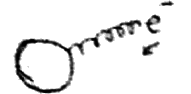
\includegraphics[width=0.2\textwidth]{./images/1-lorentz-model}
	\caption{Diagram of the Lorentz model for an atom}
	\label{fig:lorentz-model}
\end{figure}

Therefore, the equation of motion for the electron is
\begin{align*}
	\ddot{x} + \omega_{0}^{2}x = 0 \qc \omega_{0} = \sqrt{\frac{k}{m}} \Rightarrow x = A \cos(\omega_{0} t + \varphi)
\end{align*}
Introducing a damping term to account for the spontaneous emission, we get
\begin{align}
	\ddot{x} + \gamma \dot{x} + \omega_{0}^{2}x = 0
\end{align}

%-----------------------------------------------------------------
\subsection[Electric dipole approximation]{Electric dipole approximation (EDA)}
In the presence of an external electric field, $\va{E}(z,t) = E_{0} \cos(kz - \omega t) \vu{x}$, and introducing the oscillator strength, $f$, we can explain absorption and stimulated emission as well.

\begin{defi}[Oscillator strength]
	The oscillator strength, $f$, is a dimensionless quantity that expresses the probability of absorption or emission of electromagnetic radiation in transitions between energy levels of an atom or molecule.
	\begin{align*}
		f &> 0 \Rightarrow \text{ absorption} \\
		f &< 0 \Rightarrow \text{ stimulated emission}
	\end{align*}
\end{defi}

The force that acts upon a charged particle in the presence of an electric field is $\va{F} = q \va{E}$, therefore, we get
\begin{align*}
	\ddot{x} + \gamma \dot{x} + \omega_{0}^{2}x = f \frac{e E_{0}}{m} \cos(kz - \omega t)
\end{align*}

We can assume that the size of the atom is much smaller than the optical wavelength, so that the electron only sees the field at the nuclear position; this approximation is the so called electric dipole approximation. Therefore, $k z_{cm} \to 0$, and the previous equation becomes
\begin{align}
	\ddot{x} + \gamma \dot{x} + \omega_{0}^{2}x = f \frac{e E_{0}}{m} \cos(\omega t)
\end{align}

Consequently, we can get absorption or stimulated emission. Since $\dv*{W}{t} = - P$, we can study them measuring the mean value of the power in a cycle:
\begin{align}
	\ev{P} = \ev{F \dot{x}}
	\begin{cases}
		>0 & \text{(absorption)} \\
		<0 & \text{(stimulated emission)}
	\end{cases}
\end{align}
This models gives us $x(t)$.

\subsubsection*{Susceptibility}
In a homogeneous linear and isotropic dielectric medium, the polarization is aligned with and proportional to the electric field: $\va{P} = \varepsilon_{0} \chi \va{E}$. In a dipole, it can be written as $P = N e x$. Therefore, we can express the susceptibility as
\begin{align}
	\chi = \frac{N e x}{\varepsilon E} \equiv \chi' + i \chi''
\end{align}
The real part of the susceptibility, $\Re{\chi} = \chi'$ is related to index of refraction of the medium; the imaginary part, $\Im{\chi} = \chi''$ is related to the absorption coefficient.

\subsubsection*{Other media}
The natural frequency, $\omega_{0}$, gives us the model of the properties of the media. For metals, for instance, $\omega_{0} \to 0$ (electrons are not bound).

%-----------------------------------------------------------------
\subsection{Classical coherence}
\subsubsection*{First-order correlation function}
We can measure the coherence of an electric field with the help of an interferometer. In the figure \ref{fig:interferometer}, we see that $\va{E}_{1} = \va{E}(t)$, $\va{E}_{2} = \va{E}(t + \tau)$, and $\va{E}_{sum} = \va{E}_{1} + \va{E}_{2}$. So that, the intensity detected is $I \propto \ev{\va{E}^{2}_{sum}}$.
\begin{figure}[H]
	\centering
	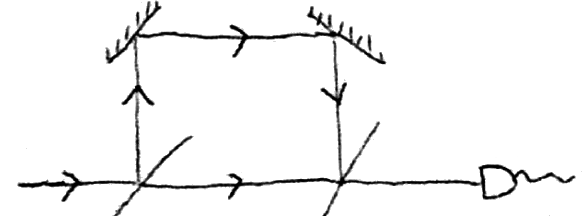
\includegraphics[width=0.5\textwidth]{./images/1-interferometer}
	\caption{Diagram of an interferometer with 50--50 beam splitters}
	\label{fig:interferometer}
\end{figure}

If we express $\va{E}(\va{r},t) = \va{E}^{(-}(\va{r},t) + \va{E}^{(-}(\va{r},t)$, where $\va{E}^{(+)} \equiv \va{E}^{(-)\sast}$, we can rewrite the expression for $I$:
\begin{flalign*}
	I & \propto \ev{(\va{E}_{1} + \va{E}_{2})^{2}} = \cdots = \ev{E^{(-)}_{1} E^{(+)}_{1}} + \ev{E^{(-)}_{2} E^{(+)}_{2}} + 2 \Re{ \ev{E^{(-)}_{1} E^{(+)}_{2}} } & \\
	& \Rightarrow I \propto 2 I_{0} + 2 \Re{E^{(-)}(t) + E^{(+)}(t + \tau)}
\end{flalign*}

\begin{defi}[First-order correlation function]
	\begin{align}
		G^{(1)}(t, t + \tau) \equiv \ev{E^{(-)}(t) + E^{(+)}(t + \tau)} = G^{(1)}(\tau)
	\end{align}
\end{defi}

The visibility is defined as $V = \dfrac{I_{max} - I_{min}}{I_{max} + I_{min}}$. Rewriting the first-order correlation function as $G^{(1)}(\tau) = \abs{G^{(1)}(\tau)} e^{i \phi(\tau)}$, we can easily work out $I_{max}$ and $I_{min}$:
\begin{flalign*}
	I & \propto 2 I_{0} + 2 \abs{G^{(1)}(\tau)} \cos[\phi(\tau)] \Rightarrow
	\begin{cases}
		I[\cos(\phi)] = -1 \Leftrightarrow I_{min} = 2I_{0} - 2 \abs{G^{(1)}(\tau)} \\
		I[\cos(\phi)] = +1 \Leftrightarrow I_{max} = 2I_{0} + 2 \abs{G^{(1)}(\tau)}
	\end{cases}
	 &
\end{flalign*}

\begin{defi}[Normalised first-order coherence function]
	We can rearrange the terms of the visibility to express it in terms of the first-order coherence function:
	\begin{align*}
		V = \dfrac{\abs{G^{(1)}(\tau)}}{\ev{E^{(-)}(t) E^{(+)}(t)}}
	\end{align*}
	this is what we call the normalised first-order coherence function, $g^{(1)}(\tau)$.
	\begin{align}
		V = \frac{I_{max} - I_{min}}{I_{max} + I_{min}} = \abs{g^{(1)}(\tau)}
		\begin{cases}
			= 0 & \Rightarrow \text{incoherent field} \\
			\in (0,1) & \Rightarrow \text{partially coherent field} \\
			= 1 & \Rightarrow \text{fully coherent field}
		\end{cases}
	\end{align}
\end{defi}

\subsubsection*{Second-order correlation function}
\begin{defi}[Normalised second-order correlation function]
	The degree of second-order correlation function is the autocorrelation function for the intensity, rather than the field. We can define this function as
	\begin{align}
		g^{(2)}(\tau) = \frac{\ev{ E^{(-)}(t) E^{(-)}(t + \tau) E^{(+)}(t + \tau) E^{(+)}(t) }}{\ev{ E^{(-)}(t) E^{(+)}(t) }}
	\end{align}
\end{defi}

%-----------------------------------------------------------------
\subsection{Hanbury--Brown--Twiss experiment}
One important feature of the second-order coherence function is that it can be measured with a reasonably simple set-up, the famous Hanbury--Brown–-Twiss apparatus (figure \ref{fig:hbt-experiment}). An input field is divided by a beam splitter, and the two components are monitored by two photo-detectors. The two detector signals are fed into a signal multiplier (mixer), though only after a variable time delay is added to one of the signals. The mixer signal is fed through a low-pass filter, which can be thought of as a integrator with a running time average.
\begin{figure}[H]
	\centering
	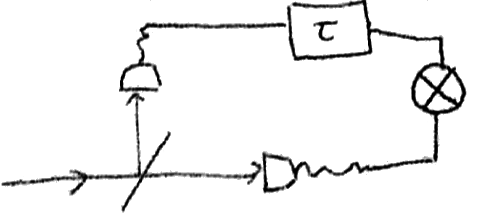
\includegraphics[width=0.4\textwidth]{./images/1-hbt-experiment}
	\caption{Diagram fo the Hanbury--Brown--Twiss experiment}
	\label{fig:hbt-experiment}
\end{figure}
This set-up, because it effectively correlates the two intensities, seems to give the $g^{(2)}(\tau)$ function as its output signal directly:
\begin{align}
	g^{(2)}(\tau) = \frac{\ev{I(t) I(t + \tau)}}{\ev{I(t)}^{2}}
\end{align}

\begin{align*}
	g^{(2)}(\tau)
	\begin{cases}
		\text{stationary field} & g^{(2)} (\tau) = 1 \\
		\text{fluctuating field} &
		\begin{cases}
			g^{(2)} (0) \geq 1 \\
			g^{(2)} (\tau) \leq g^{(2)} (0)
		\end{cases}
		\Rightarrow \text{bunching}
	\end{cases}
\end{align*}

\begin{figure}[H]
	\centering
	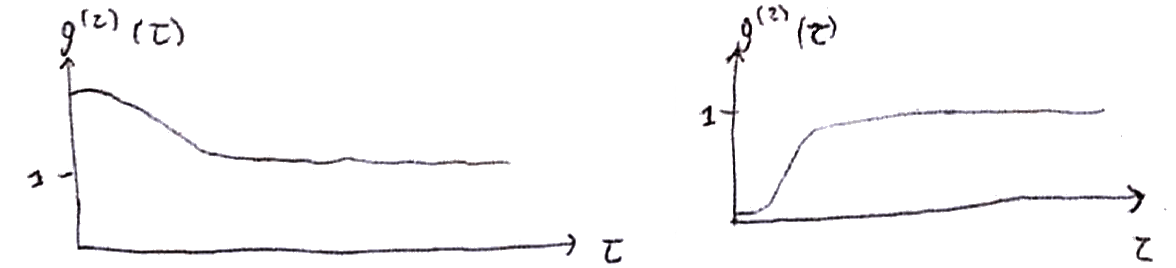
\includegraphics[width=\textwidth]{./images/1-bunching}
	\caption{(a) Bunching in a classical field, (b) antibunching in a quantum field}
	\label{fig:bunching}
\end{figure}

	%----------------------------------------------------------------------------------------
%    FUNCIONS D'UNA VARIABLE REAL
%----------------------------------------------------------------------------------------
\section{Funcions d'una variable real}
Funció real $\equiv f:D \to \mathbb{R}, \quad D \subseteq \mathbb{R}$.
\begin{itemize}
    \item Domini $\equiv \{ x \in D \mid \exists f(x) \}$.
    \item Imatge $\equiv \{ f(x) \mid x \in D \}$.
    \item Gràfic $\equiv \{ (x, f(x)) \mid x \in D \} \subseteq D \times \mathbb{R}$.
\end{itemize}

\subsubsection*{Operacions}
Siguin $f$ i $g$ funcions definides a $D$ i $E$ respectivament,
\begin{itemize}
    \item Suma: $(f+g)(x) \equiv f(x) + g(x), \quad \forall x \in D \cap E$.
    \item Producte: $(fg)(x) \equiv f(x) g(x), \quad \forall x \in D \cap E$.
    \item Composició: $(g \circ f)(x) \equiv g(f(x)), \quad \forall x \in D,$ tal que $f(x) \in E$.
\end{itemize}

%----------------------------------------------------------------------------------------
\subsection{Límit d'una funció}
$\lim\limits_{x \to a} = l$, si $\forall \varepsilon > 0, \quad \exists \delta > 0$ tal que si $|x-a| < \delta \Rightarrow |f(x) - l | < \varepsilon \Leftrightarrow$ és possible expressar una inequació entre $\delta$ i $\varepsilon$. 
L'existència del límit no depèn del comportament de $f(x)$ en $a$, sinó al seu voltant.

\subsubsection*{Propietats}
\begin{itemize}
    \item El $\lim f(x)$ és únic.
    \item Si $\exists \lim\limits_{x \to a} f(x) \Rightarrow f$ és fitada en algun $\varepsilon ^{\ast} (a, \delta)$.
    \item Si $\lim\limits_{x \to a} f(x) = k$ i $\lim\limits_{x \to a} g(x) = l$,
    \begin{itemize}
        \item $\lim (f(x) + g(x)) = k + l$.
        \item $\lim (f(x) g(x)) = kl$.
        \item $\lim (\sfrac{f(x)}{g(x)}) = \sfrac{k}{l}$ (si $l \neq 0$ i $g(x) \neq 0$ en $\varepsilon ^{\ast} (a, \delta)$.
        \item $f (x) \leq g(x)$ en algun $\varepsilon ^{\ast} (a, \delta) \Rightarrow k \neq l$.
    \end{itemize}
\end{itemize} 

\subsubsection*{Límits per la dreta i per l'esquerra (procediment)}
\begin{itemize}
    \item Dreta: $ x = a + \delta , \quad \lim\limits_{x \to a^{+}} \Rightarrow \lim\limits_{\delta \to 0^{-}} $.
    \item Esquerra: $ x = a - \delta , \quad \lim\limits_{x \to a^{-}} \Rightarrow \lim\limits_{\delta \to 0^{+}} $.
\end{itemize}

%----------------------------------------------------------------------------------------
\subsection{Continuïtat d'una funció}
Si $x \in \varepsilon (a, \delta) \Rightarrow f(x) \in \varepsilon (f(a), \varepsilon ) \Rightarrow \lim\limits_{x \to a} f(x) = f(\lim\limits_{x \to a} x)$.

\subsubsection*{Discontinuïtats}
\begin{itemize}
    \item Evitables: Quan $\exists \lim\limits_{x \to a} f(x)$ finit, però $\neq f(a)$. La discontinuïtat es pot eliminar igualant $f(a)$ a $\lim\limits_{x \to a} f(x)$.
    \item Inevitables: $\lim\limits_{x \to a} f(x)$ és $\pm \infty$ o $\nexists \lim\limits_{x \to a} f(a)$.
    \begin{itemize}
        \item De salt: $\lim\limits_{x \to a^{-}} f(x) \neq \lim\limits_{x \to a^{+}} f(x)$.
        \item Oscil·lant: $\nexists$ algun o els dos límits laterals, però $f$ és fitada a $\varepsilon ^{\ast} (a, \varepsilon)$.
        \item Infinita: $f$ no és fitada a cap $\varepsilon ^{\ast} (a, \delta)$, tant si no existeixen els límits laterals com si són infinits.
    \end{itemize}
\end{itemize}

\subsubsection*{Teorema del màxim i el mínim}
Si $f$ és contínua al compacte $K \Rightarrow f(K)$ té màxim i mínim.

\subsubsection*{Teorema del valor intermedi de Bolzano}
Si $f$ és contínua a $[a,b]$, amb $f(a) \neq f(b)$ i $y_{0} \in (f(a),f(b)) \Rightarrow \exists! c \in (a,b)$ tal que $f(c) = y_{0}$. 

\subsubsection*{Teorema de la continuïtat de la funció inversa}
Si $f$ és invertible a l'interval $I \Rightarrow f$ creix o decreix estrictament a $I$ i $f^{-1}$ és contínua a $f(I)$.

\subsubsection*{Continuïtat uniforme}
$f$ és uniformement contínua si $\forall \varepsilon > 0, \quad \exists \delta > 0$ tal que $\frac{f(x) - f(x')}{x - x'} < \frac{\varepsilon}{\delta}$.

\subsubsection*{Funció de Lipschitz}
És útil en molts casos (no sempre) per establir si una $f$ és uniformement contínua en un interval.
\begin{align*}
\begin{gathered}
    \text{Lipschitz } \Rightarrow \text{ uniformement contínua.} \\
    \text{No Lipschitz } \not \Rightarrow \text{ no uniformement contínua.}
\end{gathered}
\end{align*}
Sigui $f: A \rightarrow \mathbb{R}$. Si $\exists k \geq 0$ tal que $\displaystyle \frac{| f(a_{1}) - f(a_{2})|}{|a_{1} - a_{2}|} \leq k, \quad \forall a_{1}, a_{2} \in A$, amb $a_{1} \neq a_{2} \Rightarrow f$ és uniformement contínua a $A$.

%----------------------------------------------------------------------------------------
\subsection{Infinitèsims}
$f(x)$ és un infinitèsim quan $x \to a \Leftrightarrow \lim\limits_{x \to a} f(x) = 0$.

Si $f(x)$ i $g(x)$ són dos infinitèsims quan $x \to a$, 
\begin{align}
    \lim\limits_{x \to a} = 
    \begin{cases} 
        0 \quad \rightarrow f(x) \text{ és d'ordre superior a } g(x) \\ 
        k \quad \rightarrow f(x) \text{ i } g(x) \text{ són del mateix ordre} \\ 
        \pm \infty \quad \rightarrow f(x) \text{ és d'ordre inferior a } g(x) \\ 
        \nexists \quad \rightarrow f(x) \text{ i } g(x) \text{ no són comparables}
    \end{cases}
\end{align}
Prenent $g(x) = (x-a)^{n}, \; n \in \mathbb{N}$ com a infinitèsim de referència, 
\begin{align}
    f(x) \text{ és un infinitèsim d'ordre }
        \begin{cases} 
            > n \\ 
            n \\ 
            < n 
        \end{cases} 
    \text{ si } \lim\limits_{x \to a} \frac{f(x)}{(x-a)^{n}} =  
        \begin{cases}
            0 \\
            k \\
            \pm \infty
        \end{cases}
\end{align}
Per tant, l'ordre d'un infinitèsim mesura la rapidesa amb què $f(x)$ tendeix a zero.
\begin{align}
\begin{gathered}
    f(x) \text{ d'ordre } >n \Rightarrow f(x) = o[(x-a)]^{n} \\
    f(x) \text{ d'ordre } \geq n \Rightarrow f(x) = O[(x-a)]^{n}
\end{gathered}
\end{align}

\subsubsection*{Alguns infinitèsims equivalents quan $x \to 0$}
\begin{itemize}
    \item $f(x) \approx x$.
    \item $\sin(x) \approx x$.
    \item $\tan(x) \approx x$.
    \item $1-\cos(x) \approx \frac {x^2}{2}$.
    \item $\arcsin(x) \approx x$.
    \item $\arctan (x) \approx x$.
    \item $e^{x}-1 \approx x$.
    \item $\ln(1+x) \approx x$.
\end{itemize}
	%-----------------------------------------------------------------
%    DERIVADES
%-----------------------------------------------------------------
\section{Derivades}
\subsection{Definició}
\begin{defi}
    Sigui $f(z)$ una funció de variable complexa. La seva derivada al punt $z_{0}$ es defineix com
    \begin{align}
        f'(z_{0}) = \lim_{z \to z_{0}} \frac{f(z) - f(z_{0})}{z - z_{0}} \Leftrightarrow \der{w}{z} = \lim_{\Delta z \to 0} \frac{\Delta w}{\Delta z}
    \end{align}
\end{defi}

\begin{example}\label{ex:absz2}
    Sigui $f(z) = \abs{z}^{2}$ una funció de la qual volem trobar la seva derivada.
    
    \begin{align*}
    \begin{aligned}
        \dfrac{f(z + \Delta z) - f(z)}{\Delta z} &= \dfrac{\abs{z + \Delta z}^{2} - \abs{z}^{2}}{\Delta z} = \dfrac{(z + \Delta z) (\bar{z} + \bar{\Delta z}) - z \bar{z}}{\Delta z} \\
        &= \bar{z} + \bar{\Delta z} + \dfrac{\bar{\Delta z}}{\Delta z}
    \end{aligned}
    \end{align*}
    Per estudiar com es comporta la derivada, farem dos límits diferents:
    \begin{enumerate}[i)]
        \item $\Delta x \to 0$ i $\Delta y = 0$: 
        
        $\dfrac{\bar{\Delta z}}{\Delta z} = 1 \Rightarrow f'(z_{0}) = \lim_{z \to z_{0}} \dfrac{f(z) - f(z_{0})}{z - z_{0}} = \bar{z} + z$.
        \item $\Delta x = 0$ i $\Delta y \to 0$: 
        
        $\dfrac{\bar{\Delta z}}{\Delta z} = -1 \Rightarrow f'(z_{0}) = \lim_{z \to z_{0}} \dfrac{f(z) - f(z_{0})}{z - z_{0}} = \bar{z} - z$.
    \end{enumerate}
    Així doncs, $\nexists f'(z_{0})$ si $z \neq 0$.
\end{example}

\subsubsection*{Propietats}
\begin{enumerate}[i)]
    \item Linealitat: $\displaystyle \der{}{z}\lrpar{\alpha f(z) + \beta g(z)} = \alpha f'(z) + \beta g'(z)$.
    \item Multiplicació: $\displaystyle \der{}{z} \lrpar{f(z) g(z)} = f'(z)g(z) + g'(z)f(z)$.
    \item Divisió: $\displaystyle \der{}{z} \lrpar{\frac{f(z)}{g(z)}} = \frac{f'(z) g(z) - g'(z) f(z)}{\lrpar{g(z)}^{2}}$.
    \item Composició: $\displaystyle \omega = f(z), \, W = g(\omega) \Rightarrow \der{W}{z} = \der{W}{\omega} \der{\omega}{z}$.
\end{enumerate}

%-----------------------------------------------------------------
\subsection{Condicions per a la derivabilitat}
\subsubsection*{Condicions necessàries (equacions de Cauchy--Riemann)}
Sigui $f(z) = u(x,y) + i v(x,y)$. Definim $z_{0} = x_{0} + i y_{0}$, $\Delta z = \Delta x + i \Delta y$, i $\Delta w = f(z_{0} + \Delta z) - f(z_{0})$. Llavors,
\begin{align}
    f'(z_{0}) = \lim_{\Delta z \to 0} \frac{\Delta}{\Delta z} = \lim_{(\Delta x, \Delta y) \to (0,0)} \operatorname{Re} \lrpar{\frac{\Delta}{\Delta z}} + i \operatorname{Im} \lrpar{\frac{\Delta}{\Delta z}}
\end{align}

Considerem el camí $\Delta x \to 0$ i $\Delta y = 0$ ($\Rightarrow \Delta z = \Delta x$). Llavors, tenim
\begin{itemize}
    \item $\displaystyle \lim_{\Delta z \to 0} \operatorname{Re} \dfrac{\Delta w}{\Delta z} = \lim_{\Delta x \to 0} \dfrac{u(x_{0} + \Delta x, y_{0}) - u(x_{0}, y_{0})}{\Delta x} = u_{x}(x_{0}, y_{0})$.
    \item $\displaystyle \lim_{\Delta z \to 0} \operatorname{Im} \dfrac{\Delta w}{\Delta z} = \lim_{\Delta x \to 0} \dfrac{v(x_{0} + \Delta x, y_{0}) - v(x_{0}, y_{0})}{\Delta x} = v_{x}(x_{0}, y_{0})$.
\end{itemize}
Llavors, si $\exists f'(z_{0})$ es compleix la següent relació:
\begin{align}\label{eq:c-r1}
    f'(z_{0}) = u_{x}(x_{0},y_{0}) + i v_{x}(x_{0},y_{0})
\end{align}

En canvi si considerem el camí $\Delta x = 0$ i $\Delta y \to 0$ ($\Rightarrow \Delta z = i\Delta y$), tenim
\begin{itemize}
    \item $\displaystyle \lim_{\Delta z \to 0} \operatorname{Re} \dfrac{\Delta w}{\Delta z} = \lim_{\Delta y \to 0} \dfrac{v(x_{0}, y_{0} + \Delta y) - v(x_{0}, y_{0})}{i \Delta y} = v_{y}(x_{0}, y_{0})$.
    \item $\displaystyle \lim_{\Delta z \to 0} \operatorname{Im} \dfrac{\Delta w}{\Delta z} = \lim_{\Delta y \to 0} \dfrac{u(x_{0}, y_{0} + \Delta y) - u(x_{0}, y_{0})}{i \Delta y} = - u_{y}(x_{0}, y_{0})$.
\end{itemize}
Llavors, si $\exists f'(z_{0})$ es compleix la següent relació:
\begin{align}\label{eq:c-r2}
    f'(z_{0}) = v_{y}(x_{0},y_{0}) - i u_{y}(x_{0},y_{0})
\end{align}

A partir de \eqref{eq:c-r1} i \eqref{eq:c-r1} és trivial veure que
\begin{align}\label{eq:c-r3}
    \begin{cases} u_{x}(x_{0},y_{0}) = v_{y}(x_{0},y_{0}) \\ u_{y}(x_{0},y_{0}) = - v_{x}(x_{0},y_{0}) \end{cases}
\end{align}

Les equacions \eqref{eq:c-r1}, \eqref{eq:c-r2}, i \eqref{eq:c-r3} són les equacions de Cauchy-Riemann.
\subsubsection*{Condicions suficients}
\begin{thm}
    Donada $f(z) = u(x,y) + iv(x,y)$, si $\exists f'(z_{0})$, llavors, es compleix
    \begin{align}
        \begin{cases}u_{x} = v_{y} \\ u_{y} = - v_{x} \end{cases} \Rightarrow f'(z_{0}) = u_{x} + i v_{x}
    \end{align}
\end{thm}

\begin{thm}
    Donada $f(z) = u(x,y) + iv(x,y)$, si $\exists f'(z_{0})$ definida a un entorn de radi $\varepsilon$ al punt $z_{0} = x_{0} + i y_{0}$ i que $\exists$ les derivades parcials de primer ordre de les funcions $u$ i $v$ respecte $x$ i $y$, $\forall z \in B(z_{0}, \varepsilon)$. 
    
    Si $\exists$ aquestes derivades parcials, són contínues a $z_{0}$, i satisfan Cauchy--Riemann $\Rightarrow \exists f'(z_{0})$.
\end{thm}

%-----------------------------------------------------------------
\subsection{Fórmules de derivació}
A partir de Cauch--Riemann ($u_{x} = v_{y}$ i $u_{y} = - v_{x}$) podem arribar al següent resultat:
\begin{align}
    \pder{f}{x} = - i \pder{f}{y} \Leftrightarrow \lrpar{\pder{}{x} + i \pder{}{y}} f = 0 \Leftrightarrow \frac{\partial f}{\partial z^{\star}} = 0
\end{align}

\begin{example}
    $f(z) = \abs{z}^{2} = z z^{\star} \Rightarrow \dfrac{\partial f}{\partial z^{\star}} \Rightarrow \exists f'(z)$ només per $z = 0$.
    
    Com podem veure, comparant amb el procediment dut a terme a l'exemple \ref{ex:absz2}, aquest procediment és molt útil ja que ens porta de manera trivial a la solució, mentre que la manera tradicional és considerablement més llarga.
\end{example}

\subsubsection*{Derivació en forma polar}
A partir de l'expressió en coordenades cartesianes dels nombres complexos i la seva correspondència en polars podem reexpressar les derivades parcials de primer ordre:
\begin{align}
    \begin{cases} u_{r} = v_{r} = u_{x} \Cos \theta + u_{y} \Sin \theta \\ u_{\theta} = v_{\theta} = r \lrpar{u_{y} \Sin \theta - u_{x} \Cos \theta} \end{cases} \Rightarrow \begin{cases} u_{x} = u_{r} \Cos \theta - u_{\theta} \dfrac{\Sin \theta}{r} \\ u_{y} = u_{r} \Sin \theta + u_{\theta} \dfrac{\Cos \theta}{r} \end{cases} 
\end{align}
Tanmateix podem reexpressar l'equació \eqref{eq:c-r3} de Cauchy--Riemann:
\begin{align}
    \begin{cases}r u_{r} = v_{\theta} \\ r u_{\theta} = - r v_{r} \end{cases}
\end{align}

\subsubsection*{Exemples de derivades de funcions}
\begin{itemize}
    \item $f(z) = e^{z} = e^{x} \cos y + i e^{x} \sin y \Rightarrow f'(z) = e^{z}, \quad (f: \mbb{C} \to \mbb{C})$.
    \item $f(z) = \dfrac{1}{z} \Rightarrow f'(z) = -\dfrac{1}{z^{2}}, \quad (f: \mbb{C}\backslash \lrcur{0} \to \mbb{C})$.
    \item $f(z) = \operatorname{Ln} z = \ln r + i \operatorname{Arg} z \Rightarrow f'(z) = \dfrac{1}{z}, \quad (f: \text{“}\mbb{C}\text{”} \to \mbb{C})$.
    \item $f(z) = z^{n} \Rightarrow f'(z) = n z^{n-1}, \quad (f: \mbb{C} \to \mbb{C})$.
\end{itemize}
%-----------------------------------------------------------------
\subsection{Funcions analítiques}
\begin{defi}[Funció analítica]
    Si $\exists f'(z), \; \forall z \in \mc{D}$, llavors direm que $f(z)$ és analítica a $\mc{D}$. Una funció $f(z)$ és analítica a un punt $z_{0}$ si $\exists B(z_{0}, \varepsilon) \mid \exists f'(z), \; \forall z \in B(z_{0}, \varepsilon)$.
\end{defi}
\begin{defi}[Funció entera]
    Sigui $f(z)$ una funció de variable complexa. Diem que és entera si és analítica a tot el pla $\mbb{C}$.
\end{defi}

\begin{thm}\label{thm:exists-pder-cont}
    Si $f(z)$ és analítica a un domini $\mc{D}$, llavors $\exists f^{(n)}(z)$ i són analítiques a $\mc{D}, \; \forall n$.
\end{thm}

\subsubsection*{Regla de l'Hôpital}
Siguin $f(z)$ i $g(z)$ funcions analítiques a $\mc{D}$. Si $f(z_{0}) = g(z_{0}) = 0$, i $g'(z_{0}) \neq 0$, amb $z_{0} \in \mc{D}$; llavors es compleix
\begin{align}
    \lim_{z \to z_{0}} \frac{f(z)}{g(z)} = \frac{f'(z_{0})}{g'(z_{0})}
\end{align}

\begin{defi}[Punt singular]
    Punt on la funció $f(z)$ està mal definida en algun sentit. N'hi ha de diferents tipus:
    \begin{itemize}
        \item Singularitat aïllada: punt $z = z_{0} \mid \exists \varepsilon > 0 \mid \forall z \in B^{\star}(z_{0}, \varepsilon) \; f(z)$ és analítica.
        \item Pol: si $\exists n \in \mbb{N} \mid \lim_{z \to z_{0}} \lrpar{z - z_{0}}^{n} f(z) = A \neq 0$, llavors $z = z_{0}$ és un pol d'ordre $n$. Si $n = 1$, parlem d'un pol simple.
        \item Punt de ramificació: sense entrar en més detalls, són punts singulars que no són singularitats aïllades.
        \item Singularitat essencial: no és ni pol, ni punt de ramificació, ni punt removible ($e^{\frac{1}{z-z_{0}}}$).
    \end{itemize}
\end{defi}

%-----------------------------------------------------------------
\subsection{Funcions harmòniques}
\begin{defi}[Funció harmònica]
    Diem que una funció real de dues variables reals $H(x,y)$ és una funció harmònica si $\forall (x,y) \in \mc{D} \subseteq \mbb{R}$ $\exists$ les derivades parcials de primer i segon ordre, són contínues, i $H(x,y)$ satisfà l'equació de Laplace:
    \begin{align}
        H_{xx}(x,y) + H_{yy}(x,y) = 0
    \end{align}
\end{defi}

\begin{thm}
    Si una funció de variable complexa $f(z) = u(x,y) + iv(x,y)$ és analítica a un domini $\mc{D}$, llavors $u$ i $v$ són harmòniques a $\mc{D}$.
\end{thm}

\begin{defi}[Funció harmònica conjugada]
        Siguin $u$ i $v$ funcions harmòniques a un domini $\mc{D}$ amb $u_{x} = v_{y}$ i $u_{y} = - v_{x}$. Llavors, es diu que $v$ és l'harmònica conjugada de $u$.
\end{defi}

\begin{thm}
    Una funció $f(z) = u(x,y) + iv(x,y)$ és analítica a $\mc{D}$ sí i només si $v$ és harmònica conjugada de $u$.
\end{thm}

	%-----------------------------------------------------------------
%    INTEGRALS
%-----------------------------------------------------------------
\section{Integrals}
\subsection{Definicions}
\begin{defi}[Integral de camí]
    Sigui $f(z)$ contínua $\forall z \in$ corba $\mc{C}$. Llavors es compleix
    \begin{align}
        \lim_{n \to \infty} S_{n} \equiv \int_{a}^{b} f(z) \diff z \quad  \lrpar{\text{si } \exists = \int_{\mc{C}} f(z) \diff z}
    \end{align}
    on $S_{n} \equiv \displaystyle \sum_{k=1}^{n} f(s_{k}) (z_{k} - z_{k-1})$ i $s_{k} \in [z_{k-1}, z_{k}]$.
\end{defi}

\begin{defi}[Arc]
    Qualsevol corba que uneix dos punts. En particular, als complexos, aquests es poden parametritzar: $\begin{matrix} \mbb{R} & \to & \mbb{C} \\ t & \mapsto & z(t) \end{matrix}$.
    \begin{itemize}
        \item Arc simple (o de Jordan): $z(t_{1}) \neq z(t_{2}), \quad \forall t_{1} \neq t_{2}$.
        \item Arc suau (o diferenciable): $\exists \dot{z}(t)$ contínua.
        \item Arc suau a trossos: suma finita d'arcs suaus $\equiv$ camí.
    \end{itemize}
\end{defi}

\begin{defi}[Corba tancada simple, o de Jordan]
    Arc simple excepte pel fet que $z(a) = z(b)$.
\end{defi}

\begin{thm}[de Jordan]
    Els punts de qualsevol corba tancada simple (de Jordan) són frontera de dues regions diferents ($\mc{R}_{1} \cap \mc{R}_{2} = \varnothing$):
    \begin{enumerate}[i)]
        \item $\mc{R}_{1}$ és interior i fitada ($\exists M \in \mbb{N} \mid \abs{z} < M$).
        \item $\mc{R}_{2}$ és exterior i no fitada.
    \end{enumerate}
\end{thm}

\begin{defi}[Regió connexa]
    Sigui $\mc{R}$ una regió. Si $\forall z_{1}, z_{2} \in \mc{R}$ i $\forall \mc{C}_{1}, \mc{C}_{2} \in \mc{R}$, tots dos camins amb extrems a $z_{1}$ i  $z_{2}$, la regió definida per $\mc{C}_{1}$ i $\mc{C}_{2}$ està continguda a $\mc{R}$, diem que $\mc{R}$ és simplement connexa.
    
    Si no es compleix aquesta propietat, diem que $\mc{R}$ és múltiplement connexa.
\end{defi}

\subsubsection*{Propietats}
\begin{enumerate}[i)]
    \item $\displaystyle \int_{\mc{C}} \lrpar{f(z) + g(z)} \diff z = \displaystyle \int_{\mc{C}} f(z) \diff z + \displaystyle \int_{\mc{C}} g(z) \diff z$.
    \item $\displaystyle \int_{\mc{C}} \mu \, f(z) \diff z = \mu \displaystyle \int_{\mc{C}} f(z) \diff z, \quad \forall \mu \in \mbb{C}$.
    \item $\displaystyle \int_{a}^{b} f(z) \diff z = - \int_{b}^{a} f(z) \diff z \Leftrightarrow \cwoint_{\mc{C}} f(z) \diff z = - \ctrcwoint_{\mc{C}} f(z) \diff z$.
    \item $\displaystyle \int_{a}^{b} f(z) \diff z = \int_{a}^{m} f(z) \diff z + \int_{m}^{b} f(z) \diff z$.
    \item $\displaystyle \abs{\int_{a}^{b} f(z) \diff z} \leq \int_{\mc{C}} \abs{f(z)} \abs{\diff z} \leq M \int_{\mc{C}} \abs{\diff z} = M L_{\mc{C}}$. És a dir, si $f(z)$ és contínua $\exists M \mid \forall z \in \mc{C}, \, \abs{f(z)} \leq M$.
\end{enumerate}

%-----------------------------------------------------------------
\subsection{Integrals reals de línia}
Siguin $P(x,y)$ i $Q(x,y)$ funcions reals a la corba $\mc{C}$. Llavors, tenim
\begin{align}
    \int_{\mc{C}} \lrbra{P(x,y) \diff x + Q(x,y) \diff y} = \int_{t_{i}}^{t_{f}} \lrbra{P(x,y) \dot{x} + Q(x,y) \dot{y}} \diff t
\end{align}

Sigui $f(z) = u(x,y) + iv(x,y)$ una funció de variable complexa i contínua a la corba $\mc{C}$. Llavors, tenim
\begin{align}
\begin{aligned}
    \int_{\mc{C}} f(z) \diff z &= \int_{\mc{C}} (u + iv) (\dif x + i \diff y) \\
    &= \int_{t_{i}}^{t_{f}} \lrpar{\der{x}{t} + i \der{y}{t}} \lrbra{u (x(t), y(t)) + i v (x(t), y(t))} \\
    & = \int_{\mc{C}} (u \diff x - v \diff y) + i \int_{\mc{C}} (v \diff x + u \diff y)
\end{aligned}
\end{align}

%\begin{example}
    %TODO: 3 exemples. LOL, he tirat els apunts. Queda aixó per a la posteritat.
%\end{example}
%-----------------------------------------------------------------
%\subsection{Integrals i funcions contínues}

%-----------------------------------------------------------------
\subsection{Teorema de Green i de Cauchy}
\begin{thm}
    Sigui $f(z)$ contínua a un domini $\mc{D}$. Les següents propietats són equivalents entre si:
    \begin{enumerate}[i)]
        \item $f(z)$ té una primitiva $F(z)$ a $\mc{D}$: 
        
        $\exists F(z) \mid F'(z) = f(z)$.
        \item Les integrals de $f(z)$ sobre camins continguts a $\mc{D}$, amb un punt inicial $z_{1}$, i final $z_{2}$ fixats, tenen totes el mateix valor: 
        
        $\int_{\mc{C}_{1}} f(z) \diff z = \int_{\mc{C}_{2}} f(z) \diff z$.
        \item Les integrals de $f(z)$ sobre camins tancats continguts a $\mc{D}$ tenen totes valor zero:
        
        $\int_{\mc{C}} f(z) \diff z = 0, \quad \forall \mc{C} \subset \mc{D}$.
    \end{enumerate}
    Només el podem aplicar si el domini de $f(z)$ i el de $F(z)$ és el mateix.
\end{thm}

\begin{thm}[de Green en el pla $\mbb{R}$]
    Siguin $P(x,y)$ i $Q(x,y)$ funcions reals contínues amb derivades parcials contínues a una regió $\mc{R}$ tancada per una corba $\mc{C}$. Llavors, es compleix
    \begin{align}
        \oint_{\mc{C}} \lrpar{P \diff x + Q \diff y} = \iint_{\mc{R}} \lrpar{\pder{Q}{x} - \pder{P}{y}} \diff x \diff y
    \end{align}
\end{thm}

\begin{thm}[de Green a $\mbb{C}$]
    Sigui $F(z,z^{\star})$ contínua i amb derivades parcials contínues a $\mc{R}$. Llavors es compleix
    \begin{align}
        \oint_{C} F(z, z^{\star}) \diff z = 2i \iint_{\mc{R}} \frac{\partial F}{\partial z^{\star}} \diff A
    \end{align}
\end{thm}

\begin{thm}[de Cauchy]
    Sigui $f(z)$ analítica en una regió $\mc{R}$ i sobre la seva frontera $\mc{C}$. Llavors, es compleix
    \begin{align}
        \oint_{\mc{C}} f(z) \diff z = 0
    \end{align}
\end{thm}

\begin{thm}
    Sigui $f(z)$ analítica en una regió separada per dues corbes simples tancades $\mc{C}$ i $\mc{C}_{1}$ (on $\mc{C}_{1} \subset \mc{R}$), i sobre $\mc{C}$ i $\mc{C}_{1}$. Llavors, es compleix
    \begin{align}
        \oint_{\mc{C}} f(z) \diff z = \oint_{\mc{C}_{1}} f(z) \diff z
    \end{align}
\end{thm}

\begin{thm}
    Sigui $f(z)$ analítica en una regió limitada per les corbes simples tancades disjuntes $\mc{C}, \mc{C}_{1}, \mc{C}_{2} \dots , \mc{C}_{n}$ (on $\mc{C}_{i} \subset \mc{R}$), i sobre aquestes corbes. Llavors, es compleix
    \begin{align}
        \oint_{\mc{C}} f(z) \diff z = \oint_{\mc{C}_{1}} f(z) \diff z + \oint_{\mc{C}_{2}} f(z) \diff z + \dots + \oint_{\mc{C}_{n}} f(z) \diff z
    \end{align}
\end{thm}

%-----------------------------------------------------------------
\subsection{Fórmula integral de Cauchy}
\begin{thm}
    Sigui $f(z)$ analítica en el domini interior $\mc{R}$ a un camí tancat simple $\mc{C}$, orientat positivament, i en tots els punts del camí. Si $z_{0} \in \mc{R}$, llavors, es compleix
    \begin{align}
        f(z_{0}) = \frac{1}{2 \pi i} \oint \frac{f(z) \diff z}{z-z_{0}}
    \end{align}
\end{thm}

\begin{lem}
    Sigui $\mc{C}$ un camí tancat simple, orientat positivament, i sigui $f(z)$ analítica a $\mc{C}$ i a dins. Sigui $z$ un punt interior del domini. Llavors, es compleix
    \begin{align*}
        f'(z) = \frac{1}{2 \pi i} \oint \frac{f(s) \diff s}{(s-z)^{2}} \quad \text{i} \quad f''(z) = \frac{1}{\pi i} \oint \frac{f(s) \diff s}{(s-z)^{3}}
    \end{align*}
\end{lem}

\begin{cor}[Fórmula de diferenciació de Cauchy]
    \begin{align}
        f^{(n)}(z) = \frac{n!}{2 \pi i} \oint \frac{f(s) \diff s}{(s-z)^{n+1}}
    \end{align}
\end{cor}

%-----------------------------------------------------------------
\subsection{Teoremes relacionats}
\begin{thm}[de Morera]
    Sigui $f(z)$ contínua en un domini $\mc{D}$. Si $\oint_{\mc{C}} f(z) \diff z = 0, \; \forall \mc{C}$ tancat (on $\mc{C} \in \mc{D}$), llavors $f(z)$ és analítica en $\mc{D}$. 
\end{thm}
Aquest teorema és una conseqüència del teorema \ref{thm:exists-pder-cont}.

\begin{lem}
    Sigui $f(z)$ analítica a l'interior i els punts d'una circumferència $\mc{C}_{R}$ centrada a $z_{0}$ i de radi $R$. Si $\abs{f(z)} \leq M_{R}, \; \forall z \in \mc{C}_{R}$, llavors, es compleix
    \begin{align}
        \abs{f^{(n)}(z)} \leq \frac{n! M_{R}}{R^{n}}
    \end{align}
\end{lem}

\begin{thm}[de Liouville]
    Una funció $f(z)$ és analítica i fitada $\forall z \in \mbb{C} \Leftrightarrow f(z)$ és constant a tot el pla complex.
\end{thm}
\begin{sproof}
    Sigui $f(z)$ una funció entera (analítica a tot $\mc{C}$). Llavors, es pot representar per la seva sèrie de Taylor al voltant de zero:
    \begin{align*}
        f(z) = \sum_{n=0}^{\infty} a_{n} z^{n}, \quad a_{n} = \frac{f^{(n)}(0)}{n!} = \frac{1}{2\pi i} \oint_{\mc{C}} \frac{f(s)}{s^{n+1}} \diff s
    \end{align*}
    on $\mc{C}$ és una circumferència centrada a $0$ de radi $r>0$. Suposem que $f$ és fitada $\Leftrightarrow \abs{f(z)} \leq M$, $\forall z$. Llavors podem estimar directament que 
    \begin{align*}
        \abs{a_{n}} \leq \frac{1}{2 \pi} \oint_{\mc{C}} \frac{ \abs{f(s)}}{\abs{s}^{n+1}} \abs{\dif s} \leq \frac{1}{2 \pi} \oint_{\mc{C}} \frac{M}{r^{n+1}} \abs{\dif s} = \frac{M}{2 \pi r^{n+1}} \oint_{\mc{C}} \abs{\dif s} = \frac{M}{2 \pi r^{n+1}} 2 \pi r = \frac{M}{r^n}
    \end{align*}
    Observem, no obstant, l'elecció de $r$ és un nombre positiu arbitrari. Així doncs, fent $r \to \infty$ fa que $a_{n} = 0$, $\forall n \geq 1$. Així doncs, $f(z) \equiv a_{0}$.
\end{sproof}
	%----------------------------------------------------------------------------------------
%    SÈRIES DE TAYLOR I LAURENT
%----------------------------------------------------------------------------------------
\section{Sèries de Taylor i Laurent}
\subsubsection*{Sèrie geomètrica}
Considerem la sèrie geomètrica: $\displaystyle \sum_{k=0}^{n} z^{k} = 1 + z + z^{2} + \dots + z^{n} = \frac{1-z^{n+1}}{1-z}$, si $z \neq 1$. Quin comportament podem esperar de la sèrie quan $n \to \infty$?
\begin{align*}
    \sum_{k=0}^{\infty} z^{k} = \frac{1}{1 - z}, \quad \abs{z} < 1
\end{align*}
Aquest resultat és particularment útil, ja que ens servirà a càlculs posteriors.

%----------------------------------------------------------------------------------------
\subsection{Sèrie de Taylor}
\begin{thm}[de Taylor]
    Sigui $g(z)$ una funció analítica en un disc $\abs{z-z_{0}} < R_{0}$, centrat a $z_{0}$ i de radi $R_{0}$. Llavors, es compleix
    \begin{align}
        g(z) = \sum_{n=0}^{\infty} a_{n} (z-z_{0})^{n}, \quad \text{amb } a_{n} = \frac{g^{(n)}(z_{0})}{n!}
    \end{align}
\end{thm}
L'expansió en sèrie de $e^{z}$, $\sin z$, i $\cos z$ també tenen la mateixa forma que tenen a $\mbb{R}$:
\begin{itemize}
    \item $\displaystyle e^{z} = \sum_{n=0}^{\infty} \frac{z^{n}}{n!}$.
    \item $\displaystyle \sin z = \frac{e^{iz} - e^{-iz}}{2i} = \frac{1}{2i} \sum_{n=0}^{\infty} \frac{(iz)^{n} - (-iz)^{n}}{n!} = \sum_{n=0}^{\infty} \frac{(-1)^{n} z^{1+2n}}{(1+2n)!}$.
    \item $\displaystyle \cos z = \frac{e^{iz} + e^{-iz}}{2} = \frac{1}{2} \sum_{n=0}^{\infty} \frac{(iz)^{n} + (-iz)^{n}}{n!} = \sum_{n=0}^{\infty} \frac{(-1)^{n} z^{2n}}{(2n)!}$.
\end{itemize}

%----------------------------------------------------------------------------------------
\subsection{Sèrie de Laurent}
\begin{thm}[de Laurent]
	Sigui $g(z)$ una funció analítica a l'anell $\mc{R} = \lrcur{z \mid R_{1} < \abs{z - z_{0}} < R_{2}}$ centrat a $z_{0}$. Sigui $\mc{C}$ qualsevol camí tancat simple, orientat positivament, que rodeja a $z_{0}$ i $\mc{C} \subset \mc{R}$. Llavors, es compleix
	\begin{align}
		g(z) &= \sum_{n=0}^{\infty} a_{n} \lrpar{z-z_{0}}^{n} + \sum_{n=1}^{\infty} \frac{b_{n}}{\lrpar{z - z_{0}}}
	\end{align}
	amb $a_{n} = \dfrac{1}{2 \pi i} \displaystyle \int_{\mc{C}} \frac{g(z) \diff z}{\lrpar{z-z_{0}}^{n+1}}$, i $b_{n} = \dfrac{1}{2 \pi i} \displaystyle \int_{\mc{C}} \frac{g(z) \diff z}{\lrpar{z-z_{0}}^{-n+1}}$.

	O alternativament
	\begin{align}
		g(z) &= \sum_{n = -\infty}^{\infty} c_{n} \lrpar{z-z_{0}}^{n}
	\end{align}
	amb $c_{n} = \dfrac{1}{2\pi i} \displaystyle \int_{\mc{C}} \frac{g(z) \diff z}{\lrpar{z-z_{0}}^{n+1}}$.
\end{thm}

\begin{example}
    \begin{itemize}
        \item $\displaystyle f(z) = e^{z} = \sum_{n_{0}}^{\infty} \frac{z^{n}}{n!}$ (Taylor).
        \item $\displaystyle f(z) = e^{1/z} = \sum_{n_{0}}^{\infty} \frac{1}{z^{n}}\frac{1}{n!}$ (Laurent).
    \end{itemize}
    Com podem veure, l'estratègia per facilitar el càlcul de les sèries de Laurent és fer Taylor i fer el canvi de variable adequat.
\end{example}

%----------------------------------------------------------------------------------------
\subsection{Residu}
\begin{defi}[Residu]
	La constant $a_{-1}$ a la sèrie de Laurent de $f(z)$ al punt $z_{0}$ s'anomena residu de $f(z)$. Ho expressem de la següent forma:
	\begin{align}
	    \underset{z=z_{0}}{\operatorname{Res}} f(z) \equiv a_{-1}
    \end{align}
	Si $f(z)$ és analítica al punt $z_{0}$, el seu residu és zero; si $z_{0}$ és una singularitat, $\underset{z=z_{0}}{\operatorname{Res}} f(z) \neq 0$.
\end{defi}

\subsubsection*{Pol simple}
Fent Laurent, tenim $f(z) = \dfrac{a_{-1}}{z-z_{0}} +a_{0} + a_{1} + \dots$. Considerem la funció $g(z) = \lrpar{z-z_{0}} f(z)$, que és analítica, per tant podem fer Taylor: $g(z) = a_{-1} + a_{0}\lrpar{z-z_{0}} + a_{1}\lrpar{z-z_{0}}^{2}$. Així doncs,
\begin{align}
	\underset{z=z_{0}}{\operatorname{Res}} f(z) = \lim_{z \to z_{0}} \lrpar{z-z_{0}} f(z)
\end{align}

\subsubsection*{Pol d'ordre $n$}
Fent Laurent, tenim $f(z) = \dfrac{a_{-n}}{\lrpar{z-z_{0}}^{n}} + \dfrac{a_{n-1}}{\lrpar{z-z_{0}}^{n-1}} + \dots + \dfrac{a_{-1}}{\lrpar{z-z_{0}}} + a_{0} + a_{1}\lrpar{z-z_{0}}$. Considerem la funció $g(z) = \lrpar{z-z_{0}}^{n} f(z)$, que és analítica, per tant podem fer Taylor: $ g(z) = \displaystyle \sum_{s=0}^{\infty} \dfrac{g^{s}(z_{0}) \lrpar{z-z_{0}}}{s!}$. Així doncs,
\begin{align}
	\underset{z=z_{0}}{\operatorname{Res}} f(z) = \lim_{z \to z_{0}} \frac{1}{(n-1)!} \der[n-1]{}{z} \lrbra{\lrpar{z-z_{0}}^{n} f(z)}
\end{align}

\begin{thm}[del residu]
	Si $\mc{C}$ és una corba tancada simple, orientada positivament, i $f(z)$ és analítica al seu interior excepte per un nombre finit de singularitats aïllades $z_{j}$ dins de $\mc{C}$ i un nombre finit de pols simples $z_{s}$ a la corba. Llavors, es compleix
	\begin{align}
		\int_{\mc{C}'} f(z) \diff z = 2\pi i \sum_{j=1}^{n} \underset{z=z_{j}}{\operatorname{Res}} f(z) + \pi i \sum_{s=1}^{m} \underset{z=z_{s}}{\operatorname{Res}} f(z)
	\end{align}
	on $\mc{C}' = \mc{C}\backslash \lrcur{\text{punts singulars } z_{s}}$.
\end{thm}

% \begin{lem}[dels arcs petits]
% \end{lem}

%----------------------------------------------------------------------------------------
\subsection{Càlcul d'integrals reals}
\subsubsection*{Integrals racionals trigonomètriques}
Sigui $G(\sin \theta, \cos \theta)$ una funció racional trigonomètrica. Llavors, la integral de $G(\theta) \mid \theta \in [0,2\pi]$ és
\begin{align}
    \int_{0}^{2\pi} G(\sin \theta, \cos \theta) \diff \theta = \oint_{\mc{C}} G\lrpar{\frac{1}{2}\lrbra{z + \frac{1}{z}}, \frac{1}{2i}\lrbra{z - \frac{1}{z}}} \frac{\dif \theta}{iz}
\end{align}
\begin{sproof}
    Fent el canvi $z = e^{i\theta} \Rightarrow \displaystyle \frac{1}{z} = e^{-i\theta}$, arribem a $\displaystyle \cos \theta = \frac{1}{2}\lrpar{z + \frac{1}{z}}$ i $\displaystyle \sin \theta = \frac{1}{2i}\lrpar{z - \frac{1}{z}}$.
\end{sproof}

\subsubsection*{Estudi dels pols simples}
Sigui $G(\theta) = \dfrac{\dif \theta}{a + b \cos \theta}$ una funció trigonomètrica racional. Llavors, podem expressar la integral sobre la corba $\abs{z} = 1$ com
\begin{align}
    \int_{0}^{2\pi} \frac{\dif \theta}{a + b \cos \theta} = \frac{2}{ib} \int_{\abs{z} = 1} \frac{\dif z}{z^{2} + 2Az + 1}, \quad \text{amb } A = \frac{a}{b}
\end{align}

\begin{sproof}
	$\displaystyle \int_{0}^{2\pi} \frac{\dif \theta}{a + b \cos \theta} = \int_{\abs{z} = 1} \frac{\dif z}{iz \lrpar{a + b \frac{z^{2}+1}{2z}}} = \frac{1}{ib} \int_{\abs{z} = 1} \frac{\dif z}{\frac{z^{2} + 1}{2} + Az} = \frac{2}{ib} \int_{\abs{z} = 1} \frac{\dif z}{z^{2} + 2Az + 1}$.
\end{sproof}
Així doncs, segons la naturalesa dels pols que tingui la funció, la seva integral tindrà un resultat o un altre. En concret, veiem que són els següents:
\begin{align}
    \int_{0}^{2\pi} \frac{\dif \theta}{a + b \cos \theta} = \begin{cases} \dfrac{2\pi}{\sqrt{a^{2} - b^{2}}}, & \lrpar{\dfrac{a}{b}}^{2} > 1 \\ 0, & \lrpar{\dfrac{a}{b}}^{2} < 1 \end{cases}
\end{align}
\begin{sproof}
    Fent $z^{2} + 2Az + 1 = 0$ trobem el següents pols simples:
    \begin{itemize}
    	\item $A^{2} > 1: z_{\pm} = -A \pm \sqrt{A^{2} -1}$.
    	    \newline $\displaystyle \dfrac{2}{ib} \int \dfrac{\dif z}{(z - z_{+})(z - z_{-})} = \dfrac{2}{ib} (2\pi i) \underset{z = z_{+}}{\operatorname{Res}} \dfrac{\dif z}{z^{2} + 2Az + 1}$
    	    \newline $\displaystyle \phantom{\dfrac{2}{ib} \int \dfrac{\dif z}{(z - z_{+})(z - z_{-})}} = \frac{2}{ib} (2\pi i) \dfrac{1}{2z_{+} + 2z{-}} = \dfrac{2\pi}{\sqrt{a^{2} - b^{2}}}$.
    	\item $A^{2} < 1: z_{\pm} = -A \pm i \sqrt{1 - A^{2}} \Rightarrow \abs{z_{\pm}} = 1$.
        	\newline Fem $a + b \cos \theta = 0 \Rightarrow \cos \theta = -\dfrac{a}{b} = - \sqrt{A} < 1$. Llavors, tenim una integral impròpia amb pols simples a la corba, i tenim
        	\newline $\displaystyle \int_{0}^{2\pi} \frac{\dif \theta}{a + b \cos \theta} = \int_{\mc{C}_{A}} \frac{\dif z}{z^{2} + 2Az + 1} = - \int_{\mc{C}_{1}} - \int_{\mc{C}_{2}}$
        	\newline $\displaystyle \phantom{\int_{0}^{2\pi} \frac{\dif \theta}{a + b \cos \theta}} = - \dfrac{\pi}{2i\sqrt{1-A^{2}}} + \dfrac{\pi}{2i \sqrt{1-A^{2}}} \equiv 0$.
    \end{itemize}
\end{sproof}

\begin{example}
    $\displaystyle \int_{0}^{2\pi} \frac{\dif \theta}{2 + \cos \theta} = -i \oint_{\abs{z}=1} \frac{2 \diff z}{z^{2} + 4z + 1} \Rightarrow$ les singularitats són $z = -2 \pm \sqrt{3}$, llavors,
    \begin{align*}
    \begin{aligned}
        \int_{0}^{2\pi} \frac{\dif \theta}{2 + \cos \theta} &= -i (2\pi i) \underset{z=-2+\sqrt{3}}{\operatorname{Res}} \lrpar{\frac{2}{z^{2} + 4z + 1}} \\
        &= \lim_{z\to -2 + \sqrt{3}} \lrbra{\lrpar{z + 2 - \sqrt{3}} \lrpar{\frac{2}{z^{2} + 4z + 1}}} \\
        &= \eval{\frac{4\pi}{2z + 4}}_{z = -2 + \sqrt{3}} = \frac{2\pi}{\sqrt{3}} = \frac{2\pi}{\sqrt{2^{2} - 1^{2}}}
    \end{aligned}
    \end{align*}
\end{example}
%--------------
\subsubsection*{Integrals reals racionals de polinomis reals}
Siguin $P(x)$ i $Q(x)$ dues funcions reals tals que $\deg{P(x)} + 2 \leq \deg{Q(x)}$. Llavors, la integral de $\dfrac{P(x)}{Q(x)} \mid x \in (-\infty, \infty)$ és
\begin{align}
    \int_{-\infty}^{\infty} \frac{P(x)}{Q(x)} \diff x = 2\pi i \sum_{\operatorname{Im}z_{j} > 0} \underset{z=z_{j}}{\operatorname{Res}} \lrpar{\frac{P(z)}{Q(z)}} + \pi i \sum_{\operatorname{Im}z_{s} > 0} \underset{z=z_{s}}{\operatorname{Res}} \lrpar{\frac{P(z)}{Q(z)}}
\end{align}
on $z_{j}$ són singularitats aïllades dins la regió tancada per la corba d'integració i $z_{s}$ pols simples a la recta real $\mbb{R}$.

\begin{figure}[H]
    \centering
    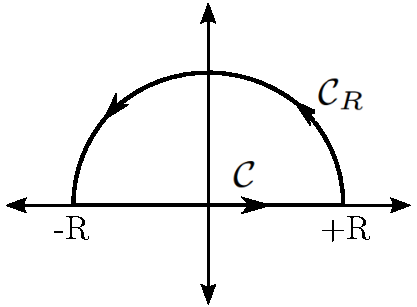
\includegraphics[width=0.3\textwidth]{./images/graph51}
    \caption{Representació gràfica dels camins sobre els quals s'integra la funció $\dfrac{P(x)}{Q(x)}$ a la demostració}
    \label{fig:graph51}
\end{figure}

\begin{sproof}
    \begin{align*}
    \begin{aligned}
        \int_{\mc{C} + \mc{C}_{R}} \frac{P(z)}{Q(z)} \diff z &= 2\pi i \sum_{\operatorname{Im}z_{j} > 0} \underset{z=z_{j}}{\operatorname{Res}} \frac{P(z)}{Q(z)} + \pi i \sum_{\operatorname{Im}z_{s} > 0} \underset{z=z_{s}}{\operatorname{Res}} \frac{P(z)}{Q(z)} \\
        &= \int_{\mc{C}} + \int_{\mc{C}_{R}} = I + I_{R}
    \end{aligned}
    \end{align*}
    Obserevem que volem trobar el valor de $I =\int_{\mc{C}} \frac{P(x)}{Q(x)} \diff x$. Fent la parametrització $z = R e^{i\theta} \Rightarrow$
    \begin{itemize}
        \item $\displaystyle \abs{I_{R}} \leq \int_{0}^{\pi} \abs{\frac{P\lrpar{Re^{i\theta}}}{Q\lrpar{Re^{i\theta}}}} R \diff \theta = \int_{0}^{\pi} \frac{\abs{z}^{m} + \dots }{\abs{z}^{m+s} + \dots} R \diff \theta = \pi \frac{R^{m+1}}{R^{m+s}} \underset{R \to 0}{\longrightarrow} 0$.
    \end{itemize}
    Llavors, tenim $\displaystyle I = \int_{\mc{C} + \mc{C}_{R}} \frac{P(z)}{Q(z)} \diff x$.
\end{sproof}

%--------------
\subsubsection*{Integrals reals racionals afegint una fase}
Siguin $P(x)$ i $Q(x)$ dues funcions reals tals que $\deg{P(x)} + 2 \leq \deg{Q(x)}$. Llavors, la integral de $\dfrac{P(x)}{Q(x)} e^{ix} \mid x \in (-\infty, \infty)$ és
\begin{align}
\begin{aligned}
    \int_{-\infty}^{\infty} \frac{P(x)}{Q(x)} e^{ix} \diff x &= 2\pi i \sum_{\operatorname{Im}z_{j} > 0} \underset{z=z_{j}}{\operatorname{Res}} \lrpar{\frac{P(z)}{Q(z)} e^{iz}} \\
    &+ \pi i \sum_{\operatorname{Im}z_{s} > 0} \underset{z=z_{s}}{\operatorname{Res}} \lrpar{\frac{P(z)}{Q(z)} e^{iz}}
\end{aligned}
\end{align}
on $z_{j}$ són singularitats aïllades dins la regió tancada per la corba d'integració i $z_{s}$ pols simples a la recta real $\mbb{R}$.

\begin{sproof}
    \begin{align*}
    \begin{aligned}
        \int_{\mc{C} + \mc{C}_{R}} \frac{P(z)}{Q(z)} e^{iz} \diff z &= 2\pi i \sum_{\operatorname{Im}z_{j} > 0} \underset{z=z_{j}}{\operatorname{Res}} \lrpar{\frac{P(z)}{Q(z)} e^{iz}} + \pi i \sum_{\operatorname{Im}z_{s} > 0} \underset{z=z_{s}}{\operatorname{Res}} \lrpar{\frac{P(z)}{Q(z)} e^{iz}} \\
        &= \int_{\mc{C}} + \int_{\mc{C}_{R}} = I + I_{R}
    \end{aligned}
    \end{align*}
    Obserevem que volem trobar el valor de $I =\int_{\mc{C}} \frac{P(x)}{Q(x)} e^{ix} \diff x$.
    \begin{itemize}
        \item $I_{R} = 0$, pel lema de Jordan.
    \end{itemize}
    Llavors, tenim $\displaystyle I = \int_{\mc{C} + \mc{C}_{R}} \frac{P(z)}{Q(z)} e^{iz} \diff x$.
\end{sproof}

\begin{lem}[de Jordan]
    Sigui $g(z)$ una funció analítica tal que $\displaystyle \lim_{\abs{z}\to \infty} \abs{g(z)} = 0$, i que $\operatorname{Im} z \geq 0$. Llavors, es compleix
    \begin{align}
        \int_{\mc{C}_{R}} g(z) e^{imz} \diff z \underset{R \to \infty}{\longrightarrow} 0, \quad m > 0
    \end{align}
\end{lem}
\begin{sproof}
    $e^{imz} = e^{imR(\Cos \theta + i \Sin \theta)} = e^{-mR\Sin \theta} e^{imR\Cos \theta}$. Observem que $e^{-mR\Sin \theta} \geq 0$ quan $\theta \in [0,\pi]$, i que $e^{imR\Cos \theta}$ no és més que una fase.

    Llavors, $\displaystyle \abs{I} \equiv \abs{\int_{\mc{C}} g(z) e^{imz} \diff z} \leq \int_{\mc{C}} \abs{g(z)} \abs{e^{imz}} \diff z$. Notem que $\sin \theta \geq \dfrac{2}{\pi} \theta$, si $\theta \in \lrbra{0,\pi / 2}$.

    $\Rightarrow \displaystyle \abs{I} \leq M_{R} \int_{0}^{\pi} \abs{e^{-mR\Sin \theta} e^{imR\Cos \theta}} R \diff \theta = 2 M_{R} R \int_{0}^{\pi/2} e^{-mR\theta /2} \diff \theta$

    $\phantom{\Rightarrow} \displaystyle \phantom{\abs{I}} = 2 M_{R} R \dfrac{\pi}{2mR} \lrpar{1 - e^{-mR}} = \dfrac{M_{R}}{m} \pi \lrpar{1 - e^{-mR}} \underset{M_{R} \to 0}{\longrightarrow} 0$.
\end{sproof}
%--------------
\subsubsection*{Integrals reals d'una funció real amb un factor de potència $\alpha$}
Sigui $R(x)$ una funció real analítica a $\mbb{C}$ tal que $\displaystyle \underset{z\to \infty}{R(z)} \to \frac{1}{z^{2+s}}$, amb $s \geq 0$, i quan $z \to 0$ $R(z)$ té com molt un pol simple. Sigui $\alpha$ un factor tal que $0 < \alpha < 1$. Llavors, la integral de $x^{\alpha} R(x) \mid x \in [0,\infty)$ és
\begin{align}
    \int_{0}^{\infty} x^{\alpha} R(x) \diff x = \frac{2\pi i}{1-e^{i 2\pi \alpha}} \sum_{z_{j} \notin \mbb{R}^{+}} \underset{z=z_{j}}{\operatorname{Res}} \lrpar{z^{\alpha}R(z)}
\end{align}
on $z_{j}$ són singularitats aïllades dins la regió tancada per la corba d'integració. Observem que la presència de pols simples a l'eix $\mc{R}$ no afecta el resultat de la integral.

\begin{figure}[H]
    \centering
    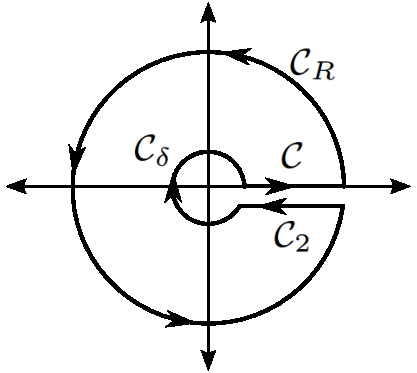
\includegraphics[width=0.3\textwidth]{./images/graph52}
    \caption{Representació gràfica dels camins sobre els quals s'integra la funció $x^{\alpha} R(x)$ a la demostració}
    \label{fig:graph52}
\end{figure}

\begin{sproof}
    \begin{align*}
    \begin{aligned}
        \int_{\mc{C} + \mc{C}_{R} + \mc{C}_{2} + \mc{C}_{\delta}} z^{\alpha}R(z) \diff z &= 2\pi i \sum_{z_{j} \notin \mbb{R}^{+}} \underset{z=z_{j}}{\operatorname{Res}} \lrpar{z^{\alpha}R(z)} \\
        &= \int_{\mc{C}} + \int_{\mc{C}_{R}} + \int_{\mc{C}_{2}} + \int_{\mc{C}_{\delta}} = I + I_{R} + I_{2} + I_{\delta}
    \end{aligned}
    \end{align*}
    Obserevem que volem trobar el valor de $I =\int_{\mc{C}} z^{a} R(z) \diff z$. Fent la parametrització $z = \rho\,e^{i\theta} \Rightarrow$
    \begin{itemize}
        \item $\displaystyle \abs{I_{R}} \leq \int_{0}^{2\pi} R^{\alpha} \abs{R\lrpar{R e^{i\theta}}} R \diff \theta = 2\pi \frac{R^{1+\alpha}}{R^{2+s}} \underset{R \to \infty}{\longrightarrow} 0$.
        \item $\displaystyle \abs{I_{\delta}} \leq \int_{2\pi}^{0} \delta^{\alpha} \abs{R \lrpar{\delta e^{i\theta}}} \delta \diff \theta = \int_{2\pi}^{0} \delta^{\alpha} \lrbra{\frac{1}{\delta} + \dots} \delta \diff \theta = - 2\pi \delta^{\alpha} \underset{\delta \to 0}{\longrightarrow} 0$.
        \item $\displaystyle I_{2} = \int_{R}^{\delta} e^{i2\pi} R\lrpar{r\,e^{i2\pi}} \lrpar{r e^{i2\pi - \varepsilon}}^{\alpha} \diff r = e^{i2\pi \alpha} \int_{R}^{\delta} r^{\alpha} R(r) \diff r = -e^{i2\pi \alpha} I$.
    \end{itemize}
    Llavors, tenim $\displaystyle I \lrpar{1-e^{i2\pi \alpha}} = 2\pi i \sum_{z_{j} \notin \mbb{R}^{+}} \underset{z=z_{j}}{\operatorname{Res}} \lrpar{z^{\alpha}R(z)}$.
\end{sproof}

	%----------------------------------------------------------------------------------------
%    SÈRIES  DE FOURIER
%----------------------------------------------------------------------------------------
\section{Sèries de Fourier}
\subsection{Definicions}
\begin{defi}[Funció periòdica]
    Diem que $f(x)$ és una funció de període $T$ si $f(x+T) \equiv f(x)$, $\forall x \in \mbb{R}$. Alternativament al període podem definir la longitud d'una funció com $L = T/2$.
\end{defi}

\begin{defi}[Sèrie de Fourier d'exponencials de període T]
    Sigui $\phi_{n}(x) = \dfrac{e^{i n \omega x}}{\sqrt{T}}$ una funció amb periodicitat $T$, amb $n \in \mbb{Z}$ i $\omega = 2\pi/T$. Es pot demostrar que $\phi_{n}(x)$ es pot aproximar com el següent sumatori, que anomenem sèrie de Fourier:
    \begin{align}\label{eq:fourier-c}
        S_{\phi_{n}}(x) = \sum_{k=-\infty}^{\infty} c_{k}\,e^{i n \omega x}, \quad c_{k} \in \mbb{C}
    \end{align}
    o de forma alternativa
    \begin{align}\label{eq:fourier-ab}
        S_{\phi_{n}}(x) = a_{0} + \sum_{k=1}^{\infty} \lrbra{a_{k} \cos \lrpar{k \omega x} + b_{k} \sin \lrpar{k \omega x}}
    \end{align}
\end{defi}
\begin{sproof} $\displaystyle \frac{1}{T} \int_{a}^{a+T} e^{im\omega x} \diff x = \delta_{0m}.$
    \begin{align*}
    \begin{aligned}
         \Rightarrow \frac{1}{T} \int_{a}^{a+T} f(x)\,e^{-ik\omega x} \diff x &= \frac{1}{T} \int_{a}^{a+T} \lrpar{\sum_{l=-\infty}^{\infty} c_{l}\,e^{il\omega x}}\,e^{-ik\omega x} \diff x \\
         &= \sum_{l=-\infty}^{\infty} c_{l} \lrpar{\frac{1}{T}  \int_{a}^{a+T} e^{i(l-k)\omega x} \diff x} = \sum_{l=\infty}^{\infty} c_{l} \delta_{lk} = c_{k}
    \end{aligned}
    \end{align*}
\end{sproof}

Les expressions \eqref{eq:fourier-c} i \eqref{eq:fourier-ab} es relacionen de la següents manera:
\begin{align*}
    \begin{cases}
        a_{0} = c_{0} \\
        a_{k} = c_{k} + c_{-k} \\
        b_{k} = i\lrpar{c_{k} - c_{-k}}
    \end{cases}
\end{align*}

\begin{thm}
    Si $f$ i $f'$ són contínues a trossos $\Rightarrow \exists \displaystyle S_{f}(x) \equiv \sum_{k=-\infty}^{\infty} c_{k}\,e^{i\omega k x}$ i es compleix que $S_{f}(x) = \displaystyle \frac{1}{2} \lim_{\varepsilon \to 0^{+}} \lrbra{f(x + \varepsilon) + f(x - \varepsilon)}$.
    
    Si $f$ i $f'$ són contínues, llavors la sèrie de Fourier $S_{f}(x)$ convergeix absolutament i uniforme a $f(x)$.
\end{thm}

\subsubsection*{Funcions parelles i senars}
\begin{defi}[Funció parella]
    Una funció parella és aquella que compleix $f(-x) = f(x)$. Un exemple típic de funció parella és $f(x) = \cos x$.
\end{defi}

\begin{defi}[Funció senar]
    Una funció senar és aquella que compleix $f(-x) = -f(x)$. Un exemple típic de funció senar és $f(x) = \sin x$.
\end{defi}

%----------------------------------------------------------------------------------------
\subsection{Sèrie de Fourier del tipus cosinus}
Sigui $f(x)$ definida a $[0,L]$. Definim $\tilde{f}(x) = \begin{cases} f(x), & x \in [0,L] \\ f(-x), & x \in [-L,0) \end{cases}$, que és una funció parella. Llavors, podem fer la sèrie de Fourier de $\tilde{f}(x)$:
\begin{align*}
\begin{gathered}
    S_{\tilde{f}}(x) = a_{0} + \sum_{n=1}^{\infty} a_{n} \cos \lrpar{\frac{n\pi x}{L}}, \quad \text{on} \\
a_{0} = \displaystyle \frac{1}{L} \int_{0}^{L} f(x) \diff x, \quad a_{n} = \frac{2}{L} \int_{0}^{L} f(x) \cos \lrpar{\frac{n \pi x}{L}} \diff x
\end{gathered}
\end{align*}
L'expressió de $S_{\tilde{f}}(x)$ és certa a $[-L,L]$ i òbviament a $[0,L]$. Llavors, es pot demostrar que $S_{\tilde{f}}(x) = f(x) \Rightarrow$
\begin{align}
    f(x) = a_{0} + \sum_{n=1}^{\infty} a_{n} \cos \lrpar{\frac{n\pi x}{L}}, \quad 0 \leq x \leq L
\end{align}

%----------------------------------------------------------------------------------------
\subsection{Sèrie de Fourier del tipus sinus}
Sigui $f(x)$ definida a $[0,L]$. Definim $\tilde{f}(x) = \begin{cases} f(x), & x \in [0,L] \\ -f(-x), & x \in [-L,0) \end{cases}$, que és una funció senar. Llavors, podem fer la sèrie de Fourier de $\tilde{f}(x)$:
\begin{align*}
    S_{\tilde{f}}(x) = \sum_{n=1}^{\infty} b_{n} \sin \lrpar{\frac{n\pi x}{L}}, \quad \text{on} \quad b_{n} = \frac{2}{L} \int_{0}^{L} f(x) \sin \lrpar{\frac{n \pi x}{L}} \diff x
\end{align*}
L'expressió de $S_{\tilde{f}}(x)$ és certa a $[-L,L]$ i òbviament a $[0,L]$. Llavors, es pot demostrar que $S_{\tilde{f}}(x) = f(x) \Rightarrow$
\begin{align}
    f(x) = \sum_{n=1}^{\infty} b_{n} \sin \lrpar{\frac{n\pi x}{L}}, \quad 0 \leq x \leq L
\end{align}

\subsubsection*{Condicions d'ortogonalitat de funcions trigonomètriques}
Les relacions següents, anomenades condicions d'ortogonalitat, poden ser de gran utilitat a l'hora de calcular els coeficients de Fourier:
\begin{itemize}
    \item $\displaystyle \int_{a}^{a+T} \cos (n\omega x) \sin (n\omega x) \diff x = 0$.
    \item $\displaystyle \int_{a}^{a+T} \cos (m\omega x) \sin (n\omega x) \diff x = \delta_{mn} \dfrac{T}{2}$.
    \item $\displaystyle \int_{a}^{a+T} \sin (m\omega x) \sin (n\omega x) \diff x = \delta_{mn} \dfrac{T}{2}$.
\end{itemize}

%----------------------------------------------------------------------------------------
\subsection{Identitat de Parseval}
\begin{thm}[de Parseval]
    Sigui $f(x) = \displaystyle a_{0} + \sum_{n=1}^{\infty} a_{n} \cos (n\omega x) + b_{n} \sin (n \omega x)$ una sèrie de Fourier, amb $\omega = \dfrac{2\pi}{T} = \dfrac{\pi}{L}$. Llavors, es compleix
    \begin{align}
        \frac{1}{T} \int_{-T/2}^{T/2} \abs{f(x)}^{2} \diff x = a_{0}^{2} + \frac{1}{2}\sum_{n=1}^{\infty} \lrpar{a_{n}^{2} + b_{n}^{2}}
    \end{align}
\end{thm}

\begin{thm}[de Parseval generalitzat]
    Siguin $f(x) = \displaystyle a_{0} + \sum_{n=1}^{\infty} a_{n} \cos (n\omega x) + b_{n} \sin (n \omega x)$ i $g(x) = \displaystyle A_{0} + \sum_{n=1}^{\infty} A_{n} \cos (n\omega x) + B_{n} \sin (n \omega x)$ sèries de Fourier, amb $\omega = \dfrac{2\pi}{T} = \dfrac{\pi}{L}$. Llavors, es compleix
    \begin{align}
        \frac{1}{T} \int_{-T/2}^{T/2} f^{\star}(x) g(x) \diff x = a_{0}^{\star} A_{0} + \frac{1}{2} \sum_{n=1}^{\infty} \lrpar{a_{n}^{\star} A_{n} + b_{n}^{\star} B_{n}}
    \end{align}
\end{thm}

\begin{sproof}
    L'identitat de Parseval es pot derivar a partir de les condicions d'ortogonalitat de les funcions sinus i cosinus.
\end{sproof}

	%----------------------------------------------------------------------------------------
%    TRANSFORMADES DE FOURIER
%----------------------------------------------------------------------------------------
\section{Transformades de Fourier}
\subsection{Definició}

\begin{defi}[Transformada de Fourier]
    Donada la funció $f(x)$, definim la seva transformada de Fourier com:
    \begin{align}
        \mc{F}\lrbra{f(x)}(k) \equiv \hat{f}(k) = \frac{1}{\sqrt{2\pi}} \int_{-\infty}^{\infty} f(x)\,e^{-ikx} \diff x
    \end{align}
\end{defi}

\begin{defi}[Transformada de Fourier inversa]
    Donada la funció $g(k)$, definim la seva transformada de Fourier inversa com:
    \begin{align}
        \mc{F}^{-1}\lrbra{g(k)}(x) \equiv \tilde{g}(x) = \frac{1}{\sqrt{2\pi}} \int_{-\infty}^{\infty} g(k)\,e^{ixk} \diff k
    \end{align}
\end{defi}

\begin{thm}
    Sigui $f(x) \in \mc{L}^{1}_{[a,b]}$ una funció tal que $f(x)$ i $f'(x)$ siguin contínues a trossos. Llavors, es compleix
    \begin{align*}
        \tilde{\hat{f}}(x) = \frac{1}{2} \lim_{\varepsilon \to 0^{+}} \lrbra{f(x + \varepsilon) + f(x - \varepsilon)} = f(x)
    \end{align*}
\end{thm}
\begin{sproof}
    \begin{align*}
    \begin{aligned}
        \tilde{\hat{f}}(x) &= \frac{1}{\sqrt{2\pi}} \int_{-\infty}^{\infty} e^{i \omega x} \lrbra{\frac{1}{\sqrt{2\pi}} \int_{-\infty}^{\infty} f(t)\,e^{-i\omega t} \diff t} \diff \omega \\
        &= \int_{-\infty}^{\infty} f(t) \lrbra{\frac{1}{2\pi} \int_{-\infty}^{\infty} e^{-i\omega (t-\omega)} \diff \omega} \diff t = \int_{-\infty}^{\infty} f(t) \delta(t-x) \diff t  = f(x)
    \end{aligned}
    \end{align*}
\end{sproof}

\begin{defi}
    $\mc{S}$ és l'espai de les funcions complexes de variable real, infinitament derivables, i que decreixen (ella i les seves derivades) més ràpidament que tota potència de $\dfrac{1}{\abs{x}}$ quan $\abs{x} \to \infty$.
\end{defi}
\begin{example}
    $f(x) \sim e^{-x^{2}} \in \mc{S}$: $e^{-x^{2}} \abs{x}^{n} \to 0$, $\forall n$.
\end{example}

\begin{thm}
    La transformada de Fourier és una operació bijectiva en l'espai $\mc{S}$, i la seva inversa és la transformada de Fourier inversa:
    \begin{align*}
        \begin{matrix}
            \mc{F}^{-1} \circ \mc{F}: & \mc{S} & \to & \mc{S} & \to & \mc{S} \\
            & \varphi & \mapsto & \hat{\varphi} & \mapsto & \tilde{\hat{\varphi}} = \varphi
        \end{matrix}
    \end{align*}
\end{thm}

\subsubsection*{Relacions de les integrals de Fourier}
\begin{example}
    Sigui $g(x) = f(x+a)$. Sabent l'expressió de $\hat{f}(k)$ podem esbrinar com es transforma $f(x)$ respecte una trasl·lació, és a dir, podem saber $\hat{g}(k)$?
    \begin{align*}
    \begin{aligned}
        \hat{g}(k) &= \frac{1}{\sqrt{2\pi}} \int_{-\infty}^{\infty} g(x)\,e^{-ikx} \diff x = \frac{1}{\sqrt{2\pi}} \int_{-\infty}^{\infty} f(x+a)\,e^{-ikx} \diff x \\
        &= \frac{1}{\sqrt{2\pi}} \int_{-\infty}^{\infty} f(\tilde{x})\,e^{-ik (\tilde{x} - a)} \diff \tilde{x} = e^{ika} \lrbra{\frac{1}{\sqrt{2\pi}} \int_{-\infty}^{\infty} f(\tilde{x})\,e^{-ik\tilde{x}} \diff \tilde{x}} \\
        &= e^{ika} \hat{f}(k)
    \end{aligned}
    \end{align*}
\end{example}
A continuació podem veure una llista de les relacions més comunes a les integrals de Fourier:
\begin{itemize}
    \item $\mc{F} \lrbra{f(x+a)} = e^{ika} \hat{f}(k)$.
    \item $\mc{F} \lrbra{e^{iax} f(x)} = \hat{f}(k-a)$.
    \item $\mc{F} \lrbra{x f(x)} = i \hat{f}'(k)$.
    \item $\mc{F} \lrbra{f'(x)} = i k \hat{f}(k)$.
    \item $\mc{F} \lrbra{f^{\star}(x)} = \hat{f}^{\star}(-k)$.
    \item $\mc{F} \lrbra{f(\lambda x)} = \dfrac{1}{\abs{\lambda}} \hat{f}\lrpar{\dfrac{k}{\lambda}}$.
    \item $\mc{F} \lrbra{f(x) \star g(x)} = \sqrt{2\pi} \hat{f}(k) \cdot \hat{g}(k)$.
    \item $\mc{F} \lrbra{f(x) \cdot g(x)} = \sqrt{2\pi} \hat{f}(k) \star \hat{g}(k)$.
\end{itemize}

%----------------------------------------------------------------------------------------
\subsection{Teorema de convolució i identitat de Parseval}
\begin{thm}[de convolució]
    Siguin $f(x)$, $g(x)$ dues funcions complexes i definim $h(x) = \displaystyle \int_{-\infty}^{\infty} f(y) g(x-y) \diff y \equiv f(x) \star g(x)$. Llavors, es compleix 
    \begin{align}
        \hat{h}(k) = \sqrt{2\pi} \hat{f}(k) \hat{g}(k)
    \end{align}
\end{thm}
\begin{sproof}
    \begin{align*}
    \begin{aligned}
        \hat{h}(k) &= \frac{1}{\sqrt{2\pi}} \int_{-\infty}^{\infty} e^{-ikx} \lrbra{\int_{-\infty}^{\infty} f(y) g(x-y) \diff y} \diff x \\ 
        &= \frac{1}{\sqrt{2\pi}} \int_{-\infty}^{\infty} f(y) g(u)\,e^{-ik(u+y)} \diff y \diff u \\
        &= \sqrt{2\pi} \lrbra{\frac{1}{\sqrt{2\pi}} \int_{-\infty}^{\infty} f(y)\,e^{-iky} \diff y} \lrbra{\frac{1}{\sqrt{2\pi}} \int_{-\infty}^{\infty} g(u)\,e^{-iku} \diff u} \\ 
        &= \sqrt{2\pi} \hat{f}(k) \hat{g}(k)
    \end{aligned}
    \end{align*}
\end{sproof}

\begin{thm}[de Parseval]
    Siguin $f(x)$ i $g(x)$ dues funcions complexes de variable real. Llavors, es compleix
    \begin{align}
        \int g^{\star}(x) f(x) \diff x = \int \hat{g^{\star}}(k) \hat{f}(k) \diff k
    \end{align}
\end{thm}

%----------------------------------------------------------------------------------------
\subsection{Transformada de Fourier del tipus cosinus}
Sigui $f(x)$ definida a $[-\infty,\infty]$. Definim $F(x) = \begin{cases} f(x), & x \geq 0 \\ f(-x), & x \leq 0 \end{cases}$, que és una funció parella. Llavors, definim la seva transformada de Fourier de tipus cosinus:
\begin{align}
    \hat{f}_{c}(\omega) \equiv \sqrt{\frac{2}{\pi}} \int_{0}^{\infty} f(x) \cos (\omega x) \diff x
\end{align}
de manera que es compleix
\begin{align}
    f(x) = \sqrt{\frac{2}{\pi}} \int_{0}^{\infty} \hat{f}_{c}(\omega) \cos (\omega x) \diff \omega
\end{align}
Observem que es conserva la paritat de la transformada: $\hat{F}(\omega) = \hat{F}(\omega)$.
\begin{sproof}
    \begin{align*}
    \begin{aligned}
        \hat{F}(\omega) &= \frac{1}{\sqrt{2}} \int_{-\infty}^{\infty} F(x)\,e^{-i\omega x} \diff x = \frac{1}{\sqrt{2}} \int_{0}^{\infty} f(x)\,e^{-i\omega x} \diff x \\ 
        &+ \frac{1}{\sqrt{2}} \int_{-\infty}^{0} f(-x)\,e^{-i\omega x} \diff x = \frac{1}{\sqrt{2}} \int_{0}^{\infty} f(x) \lrbra{e^{-i\omega x} + e^{i\omega x}} \diff x \\ 
        &= \frac{2}{\sqrt{2 \pi}} \int_{0}^{\infty} f(x) \cos (\omega x) \diff x \equiv \hat{f}_{c}(\omega)
    \end{aligned}
    \end{align*}
\end{sproof}

%----------------------------------------------------------------------------------------
\subsection{Transformada de Fourier del tipus sinus}
Sigui $f(x)$ definida a $[-\infty,\infty]$. Definim $F(x) = \begin{cases} f(x), & x > 0 \\
0, & x = 0 \\ -f(-x), & x < 0 \end{cases}$, que és una funció senar. Llavors, definim la seva transformada de Fourier de tipus sinus:
\begin{align}
    \hat{f}_{s}(\omega) \equiv \sqrt{\frac{2}{\pi}} \int_{0}^{\infty} f(x) \sin (\omega x) \diff x
\end{align}
de manera que es compleix
\begin{align}
    f(x) = \sqrt{\frac{2}{\pi}} \int_{0}^{\infty} \hat{f}_{s}(\omega) \sin (\omega x) \diff \omega
\end{align}
% Observem que $\hat{F}(k) = \pm i \hat{f}_{s}(\omega).

%----------------------------------------------------------------------------------------
\subsection{Transformada de Fourier de més d'una variable}
\begin{defi}
    Sigui $f(\vec{x})$ una funció complexa de varies variables reals. Llavors definim la seva transformada de Fourier com
    \begin{align}
        \hat{f}(\vec{k}) = \frac{1}{(2\pi)^{n/2}} \int_{\mbb{R}^{n}} f(\vec{x})\,e^{-i \omega \vec{x}} \diff^{n} \vec{x}
    \end{align}
    i compleix les següents propietats:
    \begin{enumerate}[i)]
        \item $\mc{F}\lrbra{\partial_{j} f(\vec{x})}(\vec{k}) = i k_{j} f(\vec{k})$.
        \item $\mc{F}\lrbra{\partial_{j_{1}, \dots, j_{m}} f(\vec{x})}(\vec{k}) = (i)^{m} k_{j_{1}} \dots k_{j_{m}} f(\vec{k})$.
        \item $\displaystyle \mc{F}\lrbra{f(\mat{A} \vec{x})}(\vec{k}) = \frac{1}{\det \mat{A}} \hat{f}\lrpar{(\mat{A}^{-1})^{t} \vec{k}}$.
    \end{enumerate}
\end{defi}

%----------------------------------------------------------------------------------------
\subsection{Delta de Dirac}
\begin{defi}[Delta de Dirac]
    Sigui $f(x) = \dfrac{1}{\sqrt{2\pi}} \exp \lrbra{-\dfrac{x^{2}}{2a^{2}}}$ una gaussiana. Considerem la seva transformada de Fourier:
    \begin{align}
        \hat{f}_{a}(k) = \frac{1}{\sqrt{2\pi}} a \, \exp \lrbra{-\frac{k^{2}a^{2}}{2}}
    \end{align}
    Llavors es pot veure que quan $a \to \infty$, $\hat{f}_{a}(k) = \delta(x) \equiv$ delta de Dirac.
    \begin{align}
        \delta(x) \equiv \frac{1}{\sqrt{2\pi}} \lrbra{\frac{1}{\sqrt{2\pi}} \int_{-\infty}^{\infty} e^{-ikx} \diff k} = \frac{\mc{F}\lrbra{1}(x)}{\sqrt{2\pi}}
    \end{align}
\end{defi}

De l'expressió integral de la delta de Dirac podem fer les següents observacions:
\begin{enumerate}[i)]
    \item $\displaystyle \int_{-\infty}^{\infty} \hat{f}_{a}(y) \diff y = 1$.
    \item $\displaystyle \int_{-\infty}^{\infty} \hat{f}_{a}(y) y^{2n+1} \diff y = 0$, $n \in \mbb{N}$.
    \item $\displaystyle \int_{-\infty}^{\infty} \hat{f}_{a}(y) y^{2n} \diff y = \frac{\#}{a^{2n}}$.
    \item $\displaystyle \int_{-\infty}^{\infty} \delta(y) g(y) \diff y \equiv g(0)$, quan $a \to \infty$.
\end{enumerate}

%----------------------------------------------------------------------------------------
\subsection{Aplicacions de la delta de Dirac}
\subsubsection*{Equació de Poisson}
\begin{defi}[Equació de Poisson]
    \begin{align}
        \vnabla^{2} \phi(\vec{x}) = - 4 \pi \rho(\vec{x})
    \end{align}
    La solució de l'equació d'ona és $\phi(\vec{x}) = \dfrac{q}{\abs{\vec{x} - \vec{a}}}$.
\end{defi}
\begin{sproof}
    \begin{align*}
    \begin{aligned}
        \phi(\vec{x}) &\equiv - \int 4\pi \rho(\vec{x}') G(\vec{x} - \vec{x}') \diff^{3} \vec{x}' \\
        \Rightarrow \vnabla^{2} \phi(\vec{x}) & = - \int 4\pi \rho(\vec{x}') \lrpar{\vnabla^{2} G(\vec{x} - \vec{x}')} \diff^{3} \vec{x}' = - 4 \pi \rho(\vec{x})
    \end{aligned}
    \end{align*}
    on $G(\vec{x})$ s'anomena funció de Green. Considerem la seva transformada de Fourier:
    \begin{align*}
        \hat{G}(\vec{k}) = \frac{1}{\lrpar{2\pi}^{3/2}} \int e^{-i \vec{k}\cdot \vec{y}} G(\vec{y}) \diff^{3} \vec{y} \Rightarrow G(\vec{x} - \vec{x}') = \frac{1}{\lrpar{2\pi}^{3/2}} \int e^{i \vec{k}\cdot (\vec{x} - \vec{x}')} \hat{G}(\vec{k}) \diff^{3} \vec{k}
    \end{align*}
    Calculant explícitament $\vnabla^{2} G(\vec{x} - \vec{x}')$ i fent la seva transformada de Fourier inversa podem arribar a l'expressió $\hat{G}(\vec{k}) = \dfrac{1}{(2\pi)^{3/2}} \frac{1}{\vec{k}^{2}}$. Coneguda aquesta expressió podem trobar $G(\vec{x} - \vec{x}')$ fent la seva transformada inversa:
    \begin{align*}
    \begin{gathered}
        G(\vec{x} - \vec{x}') = - \frac{1}{4\pi} \frac{1}{\abs{\vec{x} - \vec{x}'}} \\
        \Rightarrow \phi(\vec{x}) = \iiint \frac{\rho(\vec{x}')}{\abs{\vec{x} - \vec{x}'}} \diff^{3} \vec{x}' =  \iiint \frac{q \, \delta^{(3)} (\vec{x}' - \vec{a})}{\abs{\vec{x} - \vec{x}'}} \diff^{3} \vec{x}' = \frac{q}{\abs{\vec{x} - \vec{a}}}
        \end{gathered}
    \end{align*}
\end{sproof}

\subsubsection*{Equació d'ona}
\begin{defi}[Equació d'ona]
    \begin{align}
        \pder[2]{y}{x} = \frac{1}{v^{2}} \pder[2]{y}{t}
    \end{align}
    La solució de l'equació d'ona és $y(x,t) = f(x \mp vt)$.
\end{defi}
\begin{sproof}
    Coneixem les condicions inicials de la funció: $y(x, t=0)$. Primer de tot fem la transformada de Fourier de l'equació d'ona
    \begin{align*}
    \begin{aligned}
        \int_{-\infty}^{\infty} \lrpar{\pder[2]{y}{x}} e^{i\alpha x} \diff x = \frac{1}{v^{2}} \int_{-\infty}^{\infty} \lrpar{\pder[2]{y}{t}} e^{i\alpha x} \diff x
    \end{aligned}
    \end{align*}
    Considerant $\hat{y}(\alpha , t) = \dfrac{1}{\sqrt{2}} \int_{-\infty}^{\infty} y(x,t)\,e^{i\alpha x} \diff x$ i integrant per parts arribem a
    \begin{align*}
    \begin{gathered}
        (-i \alpha)^{2} \hat{y}(\alpha, t) = \frac{1}{v^{2}} \pder[2]{\hat{y}(\alpha, t)}{t} \\
        \Rightarrow \hat{y}(\alpha, t) = F(\alpha)\,e^{\pm iv\alpha t} = \hat{y}(\alpha, 0)\,e^{\pm iv\alpha t} = \lrpar{\frac{1}{\sqrt{2\pi}} \int_{-\infty}^{\infty} f(x)\,e^{i\alpha x} \diff x} e^{\pm iv \alpha t}
    \end{gathered}
    \end{align*}
    Fent la tranformada de Fourier inversa arribem a 
    \begin{align*}
        y(x,t) = \frac{1}{\sqrt{2\pi}}\int_{-\infty}^{\infty} F(\alpha)\,e^{-i \alpha (x \mp vt)} \diff \alpha = f(x \mp vt)
    \end{align*}
\end{sproof}


	%----------------------------------------------------------------------------------------
%    ALTRES RESULTATS DE VARIABLE COMPLEXA
%----------------------------------------------------------------------------------------
\section{Altres resultats de variable complexa}
\subsection{Fórmules integrals de Poisson}
Sigui un disc de radi $R$ amb punts interiors $z=r\,e^{i\theta}$, i $f(z)$ és analítica a dins el disc i la frontera. Llavors,
\begin{align}
    u(r\,e^{i\theta}) = \frac{1}{2\pi} \int_{0}^{2\pi} \frac{R^{2} - r^{2}}{R^{2} + r^{2} - 2Rr \cos(\theta - \phi)} u(Re^{i\phi}) \diff \phi
\end{align}
El mateix càlcul és vàlid per a $v(r\,e^{i\theta})$.

Sigui $f(z)$ analítica al semiplà superior del pla complex, i sigui aquesta fitada ( $\abs{f(z)} < M$ si $\abs{z} \to \infty$). Llavors,
\begin{align}
    u(x,y) = \frac{y}{\pi} \int_{-\infty}^{\infty} \frac{u(r,0)}{(r - x)^{2} + y^{2}} f(Re^{i\phi}) \diff r
\end{align}
El mateix càlcul és vàlid per a $v(x,y)$.

%----------------------------------------------------------------------------------------
\subsection{Continuació analítica}
\begin{defi}[Continuació analítica]
    Sigui $f_{0}$ una funció analítica a la regió $\mc{R}_{0}$ definida per la corba tancada simple $\mc{C}_{0}$, i sigui $f_{1}$ una funció analítica a la regió $\mc{R}_{1}$ definida per la corba tancada simple $\mc{C}_{1}$.
    
    Si $f_{0}(z) = f_{1}(z)$, $\forall z \in \mc{R}_{0} \cap \mc{R}_{1}$, diem que $f_{1}(z)$ és la continuació analítica de $f_{0}(z)$ en $\mc{R}_{0} \cup \mc{R}_{1}$.
\end{defi}
\begin{example}
    Sigui $f(z) = \displaystyle \int_{0}^{\infty} e^{-zt} \diff t = \frac{1}{z} \mid \operatorname{Re} z > 0$. Llavors $F(z) = \dfrac{1}{z}$, $\forall z \in \mbb{C} \backslash \lrcur{0}$ és la continuació analítica de $f(z)$ a $\mbb{C} \backslash \lrcur{0}$.
\end{example}

\begin{thm}[d'unicitat]
    Si $f_{1}(z)$ i $f_{2}(z)$ són analítiques en un domini $\mc{D}$ i els seus valors coincideixen sobre una successió $\lrcur{a_{k}} \to a \in \mc{D}$: $f(a_{k}) = f_{2}(a_{k})$. Llavors $f_{1}(z) = f_{2}(z)$, $\forall z \in \mc{D}$.
\end{thm}

%----------------------------------------------------------------------------------------
\subsection{Principis de reflexió d'Schwartz}
\begin{thm}
    Sigui $\mc{D}$ una regió tal que $D \cap \mbb{R} \neq \varnothing$ sigui un interval finit, i $f(z)$ sigui real $\forall z \in D \cap \mbb{R}$. Llavors, $f(z^{\star}) \equiv f^{\star}(z)$, $\forall z \in \mc{D}$.
\end{thm}
\begin{example}
    Sigui $f(z)$ una funció real, $z = x + i0$, i $x \in [-\infty, 0)$. Podem determinar l'expressió de $f(z)$, $\forall z \in \mbb{C}$ sabent les següents condicions?
    \begin{itemize}
        \item $f(z)$ és analítica a $\mbb{C} \backslash \lrbra{0,\infty}$.
        \item $f(z) \underset{\abs{z} \to 0}{\longrightarrow} 0$.
        \item $\operatorname{Im} f(x + i\varepsilon)$ és conegut (on $0 < \varepsilon \to 0$).
    \end{itemize}
    A partir de la fórmula integral de Cauchy diem, sobre la corba $\mc{C} = \mc{C}_{1} + \mc{C}_{R} + \mc{C}_{2} + \mc{C}_{\rho}$,
    \begin{align*}
    \begin{aligned}
        f(z) &= \frac{1}{2\pi i} \oint_{\mc{C}} \frac{f(\zeta)}{\zeta - z} \diff \zeta =  \oint_{\mc{C}_{1}+\mc{C}_{2}} \frac{f(\zeta)}{\zeta - z} \diff \zeta \\
        &= \frac{1}{2\pi i} \int_{0}^{\infty} \frac{f(x + i \varepsilon)}{x + i \varepsilon - z} \diff x + \frac{1}{2\pi i} \int_{\infty}^{0} \frac{f(x - i \varepsilon)}{x - i \varepsilon - z} \diff x \\
        &= \frac{1}{2\pi i} \int_{0}^{\infty} \frac{f(x + i \varepsilon) - f^{\star}(x + i \varepsilon)}{x-z} \diff x = \frac{1}{\pi} \int_{0}^{\infty} \frac{\operatorname{Im}f(x + i \varepsilon)}{x - z} \diff x
    \end{aligned}
    \end{align*}
    \begin{align*}
        \Rightarrow f(z) = \frac{1}{\pi} \int_{0}^{\infty} \frac{\operatorname{Im}f(x + i \varepsilon)}{x - z} \diff x, \quad \forall z \in \mbb{C}
    \end{align*}
\end{example}

%----------------------------------------------------------------------------------------
\subsection{Teorema de l'argument}
\begin{thm}
    Sigui $f(z)$ analítica excepte $P$ pols $\alpha_{1}, \alpha_{2}, \dots, \alpha_{P}$ d'ordre $m_{1}, m_{2}, \dots, m_{P}$, respectivament, en una regió $\mc{R}$ determinada per $\delta \mc{R} \equiv \mc{C}$. La funció $f(z)$ té alhora $N$ zeros $\beta_{1}, \beta_{2}, \dots, \beta_{N}$ d'ordre $n_{1}, n_{2}, \dots, n_{N}$, respectivament. Llavors, es compleix
    \begin{align}
        \frac{1}{2\pi i} \oint \frac{f'(z)}{f(z)} \diff z \equiv (m_{1} + m_{2} + \dots + m_{P}) - (n_{1} + n_{2} + \dots + n_{N})
    \end{align}
\end{thm}

\begin{cor}
    Sigui $f(z)$ analítica excepte $P$ pols simples ($s_{1}, s_{2}, \dots, s_{P}$) en una regió $\mc{R}$ determinada per $\delta \mc{R} \equiv \mc{C}$. La funció $f(z)$ té alhora $N$ zeros d'ordre 1 ($z_{1}, z_{2}, \dots, z_{N}$). Llavors, es compleix
    \begin{align}
        \frac{1}{2\pi i} \oint \frac{f'(z)}{f(z)} \diff z \equiv N - P
    \end{align}
\end{cor}

%\section*{Demostracions}
%\printproofs

\end{document}
